\section{Markov Decision Process for Resource Allocation}

Markov Decision Processes are used to represent how a defender may choose network nodes to support the monitoring.
While the attacker is not directly represented as an agent that will interact with the infrastructure, he can be represented in the definition of the states of the MDP and in the rewards obtained by the defender.
In this chapter, we model the migration of a Virtual Network with an MDP and represent an attacker compromising the migration process.
The solution of an MDP is a dynamic strategy that the defender should follow depending on the current state of the infrastructure (\ie the optimal policy).
We intend to convert the dynamic aspect of this policy into an \textit{a priori} deployment of the monitoring resources (\ie deploying the resources prior to the migration of the Virtual Networks).
While our MDP model could be applied to traditional networks, we have designed an attack model exploiting specificities of the SDN paradigm. 
An experimental prototype is available on github\footnote{\label{github}\url{https://github.com/FabienCharmet/MDPRA}}.



% \label{sec:mdp-reqiorements}
We formulate the following requirements regarding the formalization of the MDP:\\
\textbf{Solution form: } The solution to the problem is the optimal set of nodes to monitor the infrastructure.\\
\textbf{Constrained budgets: } The defender has a limited financial budget and a maximum performance impact threshold.
This implies that the whole infrastructure cannot be defended.\\
\textbf{Specific attacks: } The attack on the migration process must be fine grained and target specific nodes.

\begin{figure*}[htbp]


\tikzset{every picture/.style={line width=0.75pt}} %set default line width to 0.75pt        

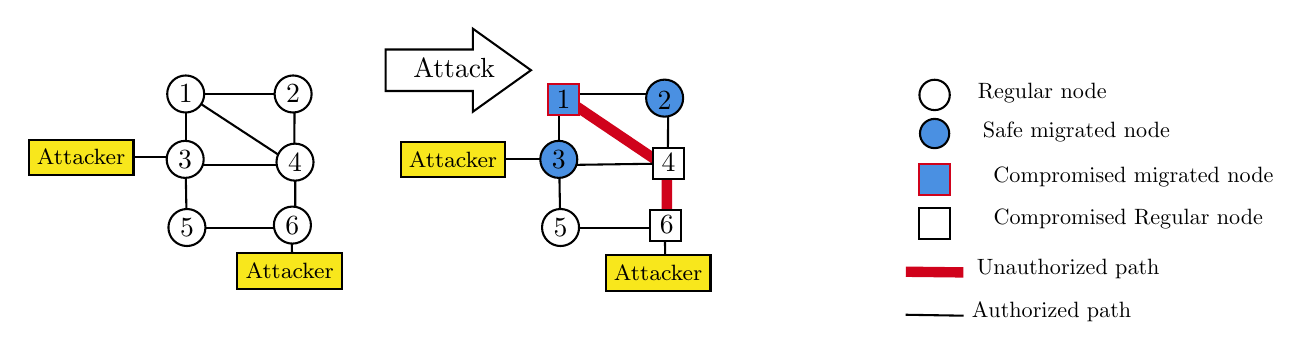
\begin{tikzpicture}[x=0.75pt,y=0.75pt,yscale=-1,xscale=1]
%uncomment if require: \path (0,300); %set diagram left start at 0, and has height of 300

%Straight Lines [id:da7739123357617682] 
\draw    (70.75,83.4) -- (108.67,83.4) ;


%Shape: Rectangle [id:dp46476407013383825] 
\draw  [fill={rgb, 255:red, 248; green, 231; blue, 28 }  ,fill opacity=1 ] (29.2,75.2) -- (79.67,75.2) -- (79.67,92.18) -- (29.2,92.18) -- cycle ;


%Straight Lines [id:da13064923443841459] 
\draw    (249.95,84.6) -- (287.87,84.6) ;


%Shape: Rectangle [id:dp28554238318371994] 
\draw  [fill={rgb, 255:red, 248; green, 231; blue, 28 }  ,fill opacity=1 ] (208.4,76.4) -- (258.87,76.4) -- (258.87,93.38) -- (208.4,93.38) -- cycle ;


%Straight Lines [id:da567285896843154] 
\draw [color={rgb, 255:red, 208; green, 2; blue, 27 }  ,draw opacity=1 ][line width=3.75]    (336.65,85.21) -- (336.67,119) ;


%Straight Lines [id:da046576842172091903] 
\draw [color={rgb, 255:red, 208; green, 2; blue, 27 }  ,draw opacity=1 ][line width=3.75]    (290.52,57.47) -- (333.33,86.33) ;


%Straight Lines [id:da5668243278416182] 
\draw    (157.33,49.22) -- (157.17,80.81) ;


%Straight Lines [id:da49434419911731065] 
\draw    (111.08,117.73) -- (149,117.73) ;


%Straight Lines [id:da6673139716829495] 
\draw    (155.58,114.06) -- (156.5,144) ;


%Straight Lines [id:da9840681038768349] 
\draw    (104.83,53.23) -- (160.58,89.73) ;


%Straight Lines [id:da4482722852442499] 
\draw    (104.83,89.73) -- (105.33,117.55) ;


%Straight Lines [id:da7670268694366985] 
\draw    (157.58,87.73) -- (157.67,119.88) ;


%Shape: Circle [id:dp667695613861877] 
\draw  [fill={rgb, 255:red, 255; green, 255; blue, 255 }  ,fill opacity=1 ] (95.92,53.23) .. controls (95.92,48.3) and (99.91,44.31) .. (104.83,44.31) .. controls (109.76,44.31) and (113.75,48.3) .. (113.75,53.23) .. controls (113.75,58.15) and (109.76,62.15) .. (104.83,62.15) .. controls (99.91,62.15) and (95.92,58.15) .. (95.92,53.23) -- cycle ;

%Shape: Circle [id:dp7262621996740888] 
\draw  [fill={rgb, 255:red, 255; green, 255; blue, 255 }  ,fill opacity=1 ] (148.58,86.06) .. controls (148.58,81.14) and (152.58,77.15) .. (157.5,77.15) .. controls (162.42,77.15) and (166.42,81.14) .. (166.42,86.06) .. controls (166.42,90.99) and (162.42,94.98) .. (157.5,94.98) .. controls (152.58,94.98) and (148.58,90.99) .. (148.58,86.06) -- cycle ;

%Shape: Circle [id:dp08856327459465119] 
\draw  [fill={rgb, 255:red, 255; green, 255; blue, 255 }  ,fill opacity=1 ] (147.33,116.4) .. controls (147.33,111.47) and (151.33,107.48) .. (156.25,107.48) .. controls (161.17,107.48) and (165.17,111.47) .. (165.17,116.4) .. controls (165.17,121.32) and (161.17,125.31) .. (156.25,125.31) .. controls (151.33,125.31) and (147.33,121.32) .. (147.33,116.4) -- cycle ;

%Straight Lines [id:da658208744911517] 
\draw    (113.75,53.23) -- (151.67,53.23) ;


%Straight Lines [id:da49379806707152474] 
\draw    (110.75,87.4) -- (148.67,87.4) ;


%Straight Lines [id:da6945831753833721] 
\draw    (104.83,62.15) -- (104.83,80.81) ;


%Shape: Circle [id:dp7034065447291917] 
\draw  [fill={rgb, 255:red, 255; green, 255; blue, 255 }  ,fill opacity=1 ] (96.52,117.56) .. controls (96.52,112.64) and (100.51,108.65) .. (105.43,108.65) .. controls (110.36,108.65) and (114.35,112.64) .. (114.35,117.56) .. controls (114.35,122.49) and (110.36,126.48) .. (105.43,126.48) .. controls (100.51,126.48) and (96.52,122.49) .. (96.52,117.56) -- cycle ;

%Shape: Circle [id:dp4778597289311547] 
\draw  [fill={rgb, 255:red, 255; green, 255; blue, 255 }  ,fill opacity=1 ] (95.67,84.73) .. controls (95.67,79.8) and (99.66,75.81) .. (104.58,75.81) .. controls (109.51,75.81) and (113.5,79.8) .. (113.5,84.73) .. controls (113.5,89.65) and (109.51,93.65) .. (104.58,93.65) .. controls (99.66,93.65) and (95.67,89.65) .. (95.67,84.73) -- cycle ;

%Shape: Circle [id:dp08437409893269954] 
\draw  [fill={rgb, 255:red, 255; green, 255; blue, 255 }  ,fill opacity=1 ] (147.67,53.23) .. controls (147.67,48.3) and (151.66,44.31) .. (156.58,44.31) .. controls (161.51,44.31) and (165.5,48.3) .. (165.5,53.23) .. controls (165.5,58.15) and (161.51,62.15) .. (156.58,62.15) .. controls (151.66,62.15) and (147.67,58.15) .. (147.67,53.23) -- cycle ;

%Shape: Circle [id:dp2544455966731902] 
\draw  [fill={rgb, 255:red, 74; green, 144; blue, 226 }  ,fill opacity=1 ] (458.61,72.28) .. controls (458.61,68.39) and (461.76,65.23) .. (465.66,65.23) .. controls (469.55,65.23) and (472.71,68.39) .. (472.71,72.28) .. controls (472.71,76.18) and (469.55,79.33) .. (465.66,79.33) .. controls (461.76,79.33) and (458.61,76.18) .. (458.61,72.28) -- cycle ;
%Straight Lines [id:da3025029961647492] 
\draw [color={rgb, 255:red, 208; green, 2; blue, 27 }  ,draw opacity=1 ][line width=3.75]    (451.78,138.87) -- (479.53,139.19) ;


%Shape: Circle [id:dp2181751678296382] 
\draw  [fill={rgb, 255:red, 255; green, 255; blue, 255 }  ,fill opacity=1 ] (458.35,53.69) .. controls (458.35,49.65) and (461.62,46.37) .. (465.66,46.37) .. controls (469.7,46.37) and (472.97,49.65) .. (472.97,53.69) .. controls (472.97,57.73) and (469.7,61) .. (465.66,61) .. controls (461.62,61) and (458.35,57.73) .. (458.35,53.69) -- cycle ;
%Straight Lines [id:da9324723367639798] 
\draw [color={rgb, 255:red, 0; green, 0; blue, 0 }  ,draw opacity=1 ]   (451.64,159.59) -- (479.68,160.05) ;


%Shape: Square [id:dp642864286437786] 
\draw  [color={rgb, 255:red, 208; green, 2; blue, 27 }  ,draw opacity=1 ][fill={rgb, 255:red, 74; green, 144; blue, 226 }  ,fill opacity=1 ] (458.16,86.93) -- (473.16,86.93) -- (473.16,101.93) -- (458.16,101.93) -- cycle ;
%Shape: Square [id:dp6103038230457687] 
\draw  [fill={rgb, 255:red, 255; green, 255; blue, 255 }  ,fill opacity=1 ] (458.16,108.16) -- (473.16,108.16) -- (473.16,123.16) -- (458.16,123.16) -- cycle ;

%Right Arrow [id:dp9004425172478334] 
\draw  [fill={rgb, 255:red, 255; green, 255; blue, 255 }  ,fill opacity=1 ] (201.2,31.78) -- (243.2,31.78) -- (243.2,21.78) -- (271.2,41.78) -- (243.2,61.78) -- (243.2,51.78) -- (201.2,51.78) -- cycle ;

%Straight Lines [id:da8396173497547912] 
\draw    (337.33,49.22) -- (337.17,80.81) ;


%Straight Lines [id:da9182383261146002] 
\draw    (291.08,117.73) -- (329,117.73) ;


%Straight Lines [id:da858414453735221] 
\draw    (335.58,114.06) -- (336,140.5) ;


%Straight Lines [id:da20295515063433045] 
\draw    (284.83,89.73) -- (285.33,117.55) ;


%Straight Lines [id:da24824224288757746] 
\draw    (293.75,53.23) -- (331.67,53.23) ;


%Straight Lines [id:da32113645413312253] 
\draw    (290.75,87.4) -- (337.58,86.73) ;


%Straight Lines [id:da20280015358357328] 
\draw    (284.83,62.15) -- (284.83,80.81) ;


%Shape: Circle [id:dp2078999158258219] 
\draw  [fill={rgb, 255:red, 255; green, 255; blue, 255 }  ,fill opacity=1 ] (276.52,117.56) .. controls (276.52,112.64) and (280.51,108.65) .. (285.43,108.65) .. controls (290.36,108.65) and (294.35,112.64) .. (294.35,117.56) .. controls (294.35,122.49) and (290.36,126.48) .. (285.43,126.48) .. controls (280.51,126.48) and (276.52,122.49) .. (276.52,117.56) -- cycle ;

%Shape: Circle [id:dp17283437144421832] 
\draw  [fill={rgb, 255:red, 74; green, 144; blue, 226 }  ,fill opacity=1 ] (275.67,84.73) .. controls (275.67,79.8) and (279.66,75.81) .. (284.58,75.81) .. controls (289.51,75.81) and (293.5,79.8) .. (293.5,84.73) .. controls (293.5,89.65) and (289.51,93.65) .. (284.58,93.65) .. controls (279.66,93.65) and (275.67,89.65) .. (275.67,84.73) -- cycle ;

%Shape: Circle [id:dp6292985525556183] 
\draw  [fill={rgb, 255:red, 74; green, 144; blue, 226 }  ,fill opacity=1 ] (326.67,55.23) .. controls (326.67,50.3) and (330.66,46.31) .. (335.58,46.31) .. controls (340.51,46.31) and (344.5,50.3) .. (344.5,55.23) .. controls (344.5,60.15) and (340.51,64.15) .. (335.58,64.15) .. controls (330.66,64.15) and (326.67,60.15) .. (326.67,55.23) -- cycle ;

%Shape: Square [id:dp21738038837827933] 
\draw  [color={rgb, 255:red, 208; green, 2; blue, 27 }  ,draw opacity=1 ][fill={rgb, 255:red, 74; green, 144; blue, 226 }  ,fill opacity=1 ] (279.37,48.2) -- (294.37,48.2) -- (294.37,63.2) -- (279.37,63.2) -- cycle ;
%Shape: Square [id:dp8476679341444072] 
\draw  [fill={rgb, 255:red, 255; green, 255; blue, 255 }  ,fill opacity=1 ] (330.08,79.23) -- (345.08,79.23) -- (345.08,94.23) -- (330.08,94.23) -- cycle ;

%Shape: Square [id:dp8795975156412624] 
\draw  [fill={rgb, 255:red, 255; green, 255; blue, 255 }  ,fill opacity=1 ] (328.48,109.23) -- (343.48,109.23) -- (343.48,124.23) -- (328.48,124.23) -- cycle ;
%Shape: Rectangle [id:dp2088885864598815] 
\draw  [fill={rgb, 255:red, 248; green, 231; blue, 28 }  ,fill opacity=1 ] (129.7,130) -- (180.17,130) -- (180.17,146.98) -- (129.7,146.98) -- cycle ;

%Shape: Rectangle [id:dp5309747919784684] 
\draw  [fill={rgb, 255:red, 248; green, 231; blue, 28 }  ,fill opacity=1 ] (307.2,131) -- (357.67,131) -- (357.67,147.98) -- (307.2,147.98) -- cycle ;


% Text Node
\draw (336.65,116) node  [align=left] {6};
% Text Node
\draw (286.87,55.7) node  [align=left] {1};
% Text Node
\draw (332.44,139.49) node  [align=left] {{\footnotesize Attacker}};
% Text Node
\draw (154.94,138.49) node  [align=left] {{\footnotesize Attacker}};
% Text Node
\draw (337.5,86.06) node  [align=left] {4};
% Text Node
\draw (335.58,56.23) node  [align=left] {2};
% Text Node
\draw (284.58,84.73) node  [align=left] {3};
% Text Node
\draw (285.43,117.56) node  [align=left] {5};
% Text Node
\draw (234.2,40.8) node  [align=left] {Attack};
% Text Node
\draw (522,158.05) node [scale=0.8] [align=left] {Authorized path};
% Text Node
\draw (530,137.33) node [scale=0.8] [align=left] {Unauthorized path};
% Text Node
\draw (559,113.58) node [scale=0.8] [align=left] {Compromised Regular node};
% Text Node
\draw (561.5,93.17) node [scale=0.8] [align=left] {Compromised migrated node};
% Text Node
\draw (534,71.48) node [scale=0.8] [align=left] {Safe migrated node};
% Text Node
\draw (517.5,52.62) node [scale=0.8] [align=left] {Regular node};
% Text Node
\draw (156.58,53.23) node  [align=left] {2};
% Text Node
\draw (104.58,84.73) node  [align=left] {3};
% Text Node
\draw (105.43,117.56) node  [align=left] {5};
% Text Node
\draw (156.25,116.4) node  [align=left] {6};
% Text Node
\draw (157.5,86.06) node  [align=left] {4};
% Text Node
\draw (104.83,53.23) node  [align=left] {1};
% Text Node
\draw (233.64,84.89) node  [align=left] {{\footnotesize Attacker}};
% Text Node
\draw (54.44,83.69) node  [align=left] {{\footnotesize Attacker}};


\end{tikzpicture}



\caption{Exfiltrating information via unauthorized routing}
\label{fig:data-exfiltration-attack}
\end{figure*}


\section{Infrastructure assumptions}
\label{sec:mdp-system-hypotheses}
We describe here the assumptions made about the infrastructure and the migration process.

% \textbf{Migration}
\begin{itemize}
    \item
    The migration will deploy in the target physical substrate all the flow rules necessary to operate the Virtual Network properly. In this chapter the expression ``migrating a node" means deploying configuration rules in a physical node.
    
    \item
    We consider that the migration of the virtual nodes is sequential~\cite{Lime-Ghorbani2014}, thus the nodes will be migrated one at a time.
    We suppose that both Virtual Network and physical infrastructure are static (\ie the topology does not change over time).
    
    \item All nodes in the original substrate have been fully compromised by the attacker and thus are not considered as candidates for the destination substrate.  
    This assumption is reinforced by the fact that forcing all the resources to be reallocated could be leveraged by the attacker in an attempt to have more nodes of the target Virtual Network relocated closer to his Virtual Machines (\ie co-residency).
    Virtual Machines are already subject to such co-residency attacks, as presented by Atya \etal in~\cite{stalling-atya2017,malicious-atya2017}.

    \item
    We also assume that the migration time is uniform across all nodes (\ie no node takes longer to migrate in the infrastructure than another).
    
    \item
     We consider the Virtual Network equivalent to the physical nodes composing its embedding.
     This assumption is used to represent how nodes will be migrated and on which physical node flow rules will be installed. 
\end{itemize}



\begin{figure*}[ht]

\tikzset{every picture/.style={line width=0.75pt}} %set default line width to 0.75pt        

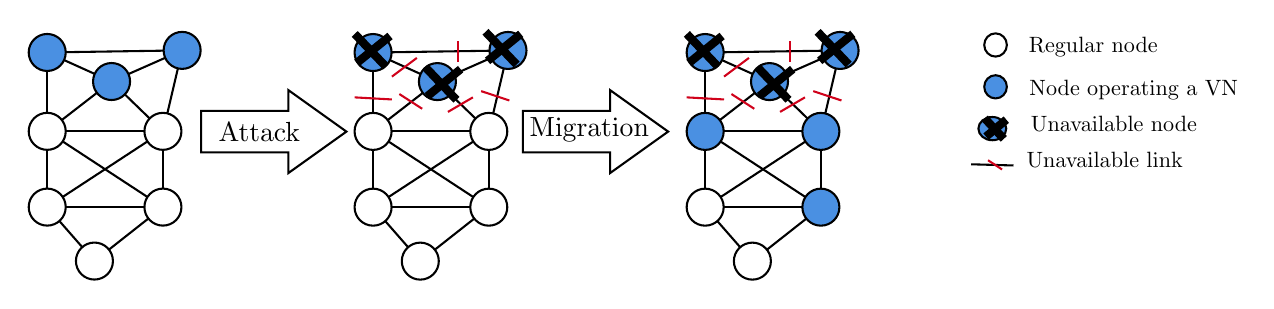
\begin{tikzpicture}[x=0.75pt,y=0.75pt,yscale=-1,xscale=1]
%uncomment if require: \path (0,300); %set diagram left start at 0, and has height of 300

%Shape: Ellipse [id:dp8430130954948494] 
\draw  [fill={rgb, 255:red, 74; green, 144; blue, 226 }  ,fill opacity=1 ] (461.48,51.56) .. controls (461.48,48.47) and (464.48,45.97) .. (468.19,45.97) .. controls (471.9,45.97) and (474.9,48.47) .. (474.9,51.56) .. controls (474.9,54.66) and (471.9,57.16) .. (468.19,57.16) .. controls (464.48,57.16) and (461.48,54.66) .. (461.48,51.56) -- cycle ;
%Shape: Ellipse [id:dp5907962461562573] 
\draw  [fill={rgb, 255:red, 74; green, 144; blue, 226 }  ,fill opacity=1 ] (464.29,31.43) .. controls (464.29,28.34) and (466.73,25.83) .. (469.74,25.83) .. controls (472.75,25.83) and (475.19,28.34) .. (475.19,31.43) .. controls (475.19,34.52) and (472.75,37.02) .. (469.74,37.02) .. controls (466.73,37.02) and (464.29,34.52) .. (464.29,31.43) -- cycle ;
%Straight Lines [id:da1514909222057811] 
\draw [color={rgb, 255:red, 0; green, 0; blue, 0 }  ,draw opacity=1 ]   (458,68.75) -- (478.38,69.32) ;


%Shape: Ellipse [id:dp8047559285598944] 
\draw  [fill={rgb, 255:red, 255; green, 255; blue, 255 }  ,fill opacity=1 ] (464.29,11.26) .. controls (464.29,8.17) and (466.73,5.67) .. (469.74,5.67) .. controls (472.75,5.67) and (475.19,8.17) .. (475.19,11.26) .. controls (475.19,14.35) and (472.75,16.86) .. (469.74,16.86) .. controls (466.73,16.86) and (464.29,14.35) .. (464.29,11.26) -- cycle ;
%Straight Lines [id:da5581047744563914] 
\draw [color={rgb, 255:red, 208; green, 2; blue, 27 }  ,draw opacity=1 ]   (472.87,71.26) -- (466.14,66.8) ;


%Straight Lines [id:da6983464143799673] 
\draw [line width=3]    (464.54,46.62) -- (473.71,56.51) ;


%Straight Lines [id:da20248481970311139] 
\draw [line width=3]    (465.15,55.41) -- (474.93,47.25) ;



%Straight Lines [id:da6176709448343998] 
\draw    (200.83,28.91) -- (225.58,52.91) ;


%Straight Lines [id:da5463688705908274] 
\draw    (200.83,28.91) -- (169.83,52.91) ;


%Straight Lines [id:da11538810799649779] 
\draw    (234.83,13.91) -- (225.92,51.91) ;


%Straight Lines [id:da8853756126147032] 
\draw    (169.83,14.91) -- (169.83,52.91) ;


%Straight Lines [id:da5031310157957251] 
\draw    (169.83,52.91) -- (225.58,89.41) ;


%Straight Lines [id:da8400043886929478] 
\draw    (169.83,89.41) -- (192.58,115.41) ;


%Straight Lines [id:da5242150334882041] 
\draw    (225.58,89.41) -- (192.58,115.41) ;


%Straight Lines [id:da3960630757961663] 
\draw    (225.58,52.91) -- (169.83,89.41) ;


%Shape: Circle [id:dp47175232960651714] 
\draw  [fill={rgb, 255:red, 255; green, 255; blue, 255 }  ,fill opacity=1 ] (160.92,52.91) .. controls (160.92,47.98) and (164.91,43.99) .. (169.83,43.99) .. controls (174.76,43.99) and (178.75,47.98) .. (178.75,52.91) .. controls (178.75,57.83) and (174.76,61.82) .. (169.83,61.82) .. controls (164.91,61.82) and (160.92,57.83) .. (160.92,52.91) -- cycle ;
%Shape: Circle [id:dp5879580381901867] 
\draw  [fill={rgb, 255:red, 255; green, 255; blue, 255 }  ,fill opacity=1 ] (216.67,52.91) .. controls (216.67,47.98) and (220.66,43.99) .. (225.58,43.99) .. controls (230.51,43.99) and (234.5,47.98) .. (234.5,52.91) .. controls (234.5,57.83) and (230.51,61.82) .. (225.58,61.82) .. controls (220.66,61.82) and (216.67,57.83) .. (216.67,52.91) -- cycle ;
%Shape: Circle [id:dp5579759383684684] 
\draw  [fill={rgb, 255:red, 255; green, 255; blue, 255 }  ,fill opacity=1 ] (160.92,89.41) .. controls (160.92,84.48) and (164.91,80.49) .. (169.83,80.49) .. controls (174.76,80.49) and (178.75,84.48) .. (178.75,89.41) .. controls (178.75,94.33) and (174.76,98.32) .. (169.83,98.32) .. controls (164.91,98.32) and (160.92,94.33) .. (160.92,89.41) -- cycle ;
%Shape: Circle [id:dp885869190555082] 
\draw  [fill={rgb, 255:red, 255; green, 255; blue, 255 }  ,fill opacity=1 ] (216.67,89.41) .. controls (216.67,84.48) and (220.66,80.49) .. (225.58,80.49) .. controls (230.51,80.49) and (234.5,84.48) .. (234.5,89.41) .. controls (234.5,94.33) and (230.51,98.32) .. (225.58,98.32) .. controls (220.66,98.32) and (216.67,94.33) .. (216.67,89.41) -- cycle ;
%Shape: Circle [id:dp3254884021888832] 
\draw  [fill={rgb, 255:red, 255; green, 255; blue, 255 }  ,fill opacity=1 ] (183.67,115.41) .. controls (183.67,110.48) and (187.66,106.49) .. (192.58,106.49) .. controls (197.51,106.49) and (201.5,110.48) .. (201.5,115.41) .. controls (201.5,120.33) and (197.51,124.32) .. (192.58,124.32) .. controls (187.66,124.32) and (183.67,120.33) .. (183.67,115.41) -- cycle ;
%Straight Lines [id:da7041582060743201] 
\draw    (178.75,52.91) -- (216.67,52.91) ;


%Straight Lines [id:da26176464493068274] 
\draw    (178.75,89.41) -- (216.67,89.41) ;


%Straight Lines [id:da45312150436944487] 
\draw    (225.58,80.49) -- (225.58,61.82) ;


%Straight Lines [id:da10497643854199257] 
\draw    (169.83,61.82) -- (169.83,80.49) ;


%Straight Lines [id:da023464273570334315] 
\draw    (169.83,14.91) -- (234.83,13.91) ;


%Straight Lines [id:da7461511731963238] 
\draw    (200.83,28.91) -- (234.83,13.91) ;


%Straight Lines [id:da6717008743630867] 
\draw    (169.83,14.91) -- (200.83,28.91) ;


%Shape: Circle [id:dp17672294199894456] 
\draw  [fill={rgb, 255:red, 74; green, 144; blue, 226 }  ,fill opacity=1 ] (160.92,14.91) .. controls (160.92,9.98) and (164.91,5.99) .. (169.83,5.99) .. controls (174.76,5.99) and (178.75,9.98) .. (178.75,14.91) .. controls (178.75,19.83) and (174.76,23.82) .. (169.83,23.82) .. controls (164.91,23.82) and (160.92,19.83) .. (160.92,14.91) -- cycle ;
%Shape: Circle [id:dp8878711028556632] 
\draw  [fill={rgb, 255:red, 74; green, 144; blue, 226 }  ,fill opacity=1 ] (191.92,28.91) .. controls (191.92,23.98) and (195.91,19.99) .. (200.83,19.99) .. controls (205.76,19.99) and (209.75,23.98) .. (209.75,28.91) .. controls (209.75,33.83) and (205.76,37.82) .. (200.83,37.82) .. controls (195.91,37.82) and (191.92,33.83) .. (191.92,28.91) -- cycle ;
%Shape: Circle [id:dp02560438280336974] 
\draw  [fill={rgb, 255:red, 74; green, 144; blue, 226 }  ,fill opacity=1 ] (225.92,13.91) .. controls (225.92,8.98) and (229.91,4.99) .. (234.83,4.99) .. controls (239.76,4.99) and (243.75,8.98) .. (243.75,13.91) .. controls (243.75,18.83) and (239.76,22.82) .. (234.83,22.82) .. controls (229.91,22.82) and (225.92,18.83) .. (225.92,13.91) -- cycle ;
%Straight Lines [id:da7816159630212767] 
\draw [color={rgb, 255:red, 208; green, 2; blue, 27 }  ,draw opacity=1 ]   (210.92,9.51) -- (210.92,19.51) ;


%Straight Lines [id:da23242280473047117] 
\draw [color={rgb, 255:red, 208; green, 2; blue, 27 }  ,draw opacity=1 ]   (221.92,33.51) -- (235.5,38.01) ;


%Straight Lines [id:da25217250177313655] 
\draw [color={rgb, 255:red, 208; green, 2; blue, 27 }  ,draw opacity=1 ]   (160.92,36.51) -- (178.92,37.51) ;


%Straight Lines [id:da8252457737222165] 
\draw [color={rgb, 255:red, 208; green, 2; blue, 27 }  ,draw opacity=1 ]   (178.92,26.51) -- (190.92,17.51) ;


%Straight Lines [id:da6307655523636441] 
\draw [color={rgb, 255:red, 208; green, 2; blue, 27 }  ,draw opacity=1 ]   (205.92,43.51) -- (217.92,36.51) ;


%Straight Lines [id:da5703265914230616] 
\draw [color={rgb, 255:red, 208; green, 2; blue, 27 }  ,draw opacity=1 ]   (193.5,42.01) -- (182.5,34.91) ;


%Straight Lines [id:da3989594608358942] 
\draw [line width=3]    (161,5.93) -- (176,21.68) ;


%Straight Lines [id:da7318288975856456] 
\draw [line width=3]    (162,19.93) -- (178,6.93) ;



%Straight Lines [id:da9963706937012238] 
\draw [line width=3]    (224,4.93) -- (239,20.68) ;


%Straight Lines [id:da43798340024618054] 
\draw [line width=3]    (225,18.93) -- (241,5.93) ;



%Straight Lines [id:da5033136183613764] 
\draw [line width=3]    (195,21.93) -- (210,37.68) ;


%Straight Lines [id:da623542865534238] 
\draw [line width=3]    (196,35.93) -- (212,22.93) ;




%Straight Lines [id:da021425369536150374] 
\draw    (43.83,28.87) -- (68.58,52.87) ;


%Straight Lines [id:da809644771756096] 
\draw    (43.83,28.87) -- (12.83,52.87) ;


%Straight Lines [id:da9075994171710501] 
\draw    (77.83,13.87) -- (68.92,51.87) ;


%Straight Lines [id:da7475460187374237] 
\draw    (12.83,14.87) -- (12.83,52.87) ;


%Straight Lines [id:da06975692875380135] 
\draw    (12.83,52.87) -- (68.58,89.37) ;


%Straight Lines [id:da9394544948671463] 
\draw    (12.83,89.37) -- (35.58,115.37) ;


%Straight Lines [id:da46361116523850066] 
\draw    (68.58,89.37) -- (35.58,115.37) ;


%Straight Lines [id:da9816638193583865] 
\draw    (68.58,52.87) -- (12.83,89.37) ;


%Shape: Circle [id:dp21531756732058427] 
\draw  [fill={rgb, 255:red, 255; green, 255; blue, 255 }  ,fill opacity=1 ] (3.92,52.87) .. controls (3.92,47.95) and (7.91,43.96) .. (12.83,43.96) .. controls (17.76,43.96) and (21.75,47.95) .. (21.75,52.87) .. controls (21.75,57.8) and (17.76,61.79) .. (12.83,61.79) .. controls (7.91,61.79) and (3.92,57.8) .. (3.92,52.87) -- cycle ;
%Shape: Circle [id:dp32258921480580105] 
\draw  [fill={rgb, 255:red, 255; green, 255; blue, 255 }  ,fill opacity=1 ] (59.67,52.87) .. controls (59.67,47.95) and (63.66,43.96) .. (68.58,43.96) .. controls (73.51,43.96) and (77.5,47.95) .. (77.5,52.87) .. controls (77.5,57.8) and (73.51,61.79) .. (68.58,61.79) .. controls (63.66,61.79) and (59.67,57.8) .. (59.67,52.87) -- cycle ;
%Shape: Circle [id:dp7783815840311967] 
\draw  [fill={rgb, 255:red, 255; green, 255; blue, 255 }  ,fill opacity=1 ] (3.92,89.37) .. controls (3.92,84.45) and (7.91,80.46) .. (12.83,80.46) .. controls (17.76,80.46) and (21.75,84.45) .. (21.75,89.37) .. controls (21.75,94.3) and (17.76,98.29) .. (12.83,98.29) .. controls (7.91,98.29) and (3.92,94.3) .. (3.92,89.37) -- cycle ;
%Shape: Circle [id:dp9106798970146953] 
\draw  [fill={rgb, 255:red, 255; green, 255; blue, 255 }  ,fill opacity=1 ] (59.67,89.37) .. controls (59.67,84.45) and (63.66,80.46) .. (68.58,80.46) .. controls (73.51,80.46) and (77.5,84.45) .. (77.5,89.37) .. controls (77.5,94.3) and (73.51,98.29) .. (68.58,98.29) .. controls (63.66,98.29) and (59.67,94.3) .. (59.67,89.37) -- cycle ;
%Shape: Circle [id:dp1831427544072476] 
\draw  [fill={rgb, 255:red, 255; green, 255; blue, 255 }  ,fill opacity=1 ] (26.67,115.37) .. controls (26.67,110.45) and (30.66,106.46) .. (35.58,106.46) .. controls (40.51,106.46) and (44.5,110.45) .. (44.5,115.37) .. controls (44.5,120.3) and (40.51,124.29) .. (35.58,124.29) .. controls (30.66,124.29) and (26.67,120.3) .. (26.67,115.37) -- cycle ;
%Straight Lines [id:da9700158448121917] 
\draw    (21.75,52.87) -- (59.67,52.87) ;


%Straight Lines [id:da010185511635833033] 
\draw    (21.75,89.37) -- (59.67,89.37) ;


%Straight Lines [id:da4677014236726348] 
\draw    (68.58,80.46) -- (68.58,61.79) ;


%Straight Lines [id:da19862578341507608] 
\draw    (12.83,61.79) -- (12.83,80.46) ;


%Straight Lines [id:da6877311034443738] 
\draw    (12.83,14.87) -- (77.83,13.87) ;


%Straight Lines [id:da39601253001890035] 
\draw    (43.83,28.87) -- (77.83,13.87) ;


%Straight Lines [id:da8270994037474519] 
\draw    (12.83,14.87) -- (43.83,28.87) ;


%Shape: Circle [id:dp2984826737185816] 
\draw  [fill={rgb, 255:red, 74; green, 144; blue, 226 }  ,fill opacity=1 ] (3.92,14.87) .. controls (3.92,9.95) and (7.91,5.96) .. (12.83,5.96) .. controls (17.76,5.96) and (21.75,9.95) .. (21.75,14.87) .. controls (21.75,19.8) and (17.76,23.79) .. (12.83,23.79) .. controls (7.91,23.79) and (3.92,19.8) .. (3.92,14.87) -- cycle ;
%Shape: Circle [id:dp6437572475375565] 
\draw  [fill={rgb, 255:red, 74; green, 144; blue, 226 }  ,fill opacity=1 ] (34.92,28.87) .. controls (34.92,23.95) and (38.91,19.96) .. (43.83,19.96) .. controls (48.76,19.96) and (52.75,23.95) .. (52.75,28.87) .. controls (52.75,33.8) and (48.76,37.79) .. (43.83,37.79) .. controls (38.91,37.79) and (34.92,33.8) .. (34.92,28.87) -- cycle ;
%Shape: Circle [id:dp23183818676236623] 
\draw  [fill={rgb, 255:red, 74; green, 144; blue, 226 }  ,fill opacity=1 ] (68.92,13.87) .. controls (68.92,8.95) and (72.91,4.96) .. (77.83,4.96) .. controls (82.76,4.96) and (86.75,8.95) .. (86.75,13.87) .. controls (86.75,18.8) and (82.76,22.79) .. (77.83,22.79) .. controls (72.91,22.79) and (68.92,18.8) .. (68.92,13.87) -- cycle ;

%Right Arrow [id:dp417684980473099] 
\draw   (87,43) -- (129,43) -- (129,33) -- (157,53) -- (129,73) -- (129,63) -- (87,63) -- cycle ;

%Right Arrow [id:dp6623970589974628] 
\draw   (242,43) -- (284,43) -- (284,33) -- (312,53) -- (284,73) -- (284,63) -- (242,63) -- cycle ;
%Straight Lines [id:da22163993557127015] 
\draw    (360.83,28.91) -- (385.58,52.91) ;


%Straight Lines [id:da8341652491193966] 
\draw    (360.83,28.91) -- (329.83,52.91) ;


%Straight Lines [id:da14662408338887967] 
\draw    (394.83,13.91) -- (385.92,51.91) ;


%Straight Lines [id:da1054361182628697] 
\draw    (329.83,14.91) -- (329.83,52.91) ;


%Straight Lines [id:da878058282787745] 
\draw    (329.83,52.91) -- (385.58,89.41) ;


%Straight Lines [id:da5143639640863213] 
\draw    (329.83,89.41) -- (352.58,115.41) ;


%Straight Lines [id:da38106162801473] 
\draw    (385.58,89.41) -- (352.58,115.41) ;


%Straight Lines [id:da9515281954413589] 
\draw    (385.58,52.91) -- (329.83,89.41) ;


%Shape: Circle [id:dp7012949201072771] 
\draw  [fill={rgb, 255:red, 74; green, 144; blue, 226 }  ,fill opacity=1 ] (320.92,52.91) .. controls (320.92,47.98) and (324.91,43.99) .. (329.83,43.99) .. controls (334.76,43.99) and (338.75,47.98) .. (338.75,52.91) .. controls (338.75,57.83) and (334.76,61.82) .. (329.83,61.82) .. controls (324.91,61.82) and (320.92,57.83) .. (320.92,52.91) -- cycle ;
%Shape: Circle [id:dp8511635916765001] 
\draw  [fill={rgb, 255:red, 74; green, 144; blue, 226 }  ,fill opacity=1 ] (376.67,52.91) .. controls (376.67,47.98) and (380.66,43.99) .. (385.58,43.99) .. controls (390.51,43.99) and (394.5,47.98) .. (394.5,52.91) .. controls (394.5,57.83) and (390.51,61.82) .. (385.58,61.82) .. controls (380.66,61.82) and (376.67,57.83) .. (376.67,52.91) -- cycle ;
%Shape: Circle [id:dp10253503783482376] 
\draw  [fill={rgb, 255:red, 255; green, 255; blue, 255 }  ,fill opacity=1 ] (320.92,89.41) .. controls (320.92,84.48) and (324.91,80.49) .. (329.83,80.49) .. controls (334.76,80.49) and (338.75,84.48) .. (338.75,89.41) .. controls (338.75,94.33) and (334.76,98.32) .. (329.83,98.32) .. controls (324.91,98.32) and (320.92,94.33) .. (320.92,89.41) -- cycle ;
%Shape: Circle [id:dp7321236156986349] 
\draw  [fill={rgb, 255:red, 74; green, 144; blue, 226 }  ,fill opacity=1 ] (376.67,89.41) .. controls (376.67,84.48) and (380.66,80.49) .. (385.58,80.49) .. controls (390.51,80.49) and (394.5,84.48) .. (394.5,89.41) .. controls (394.5,94.33) and (390.51,98.32) .. (385.58,98.32) .. controls (380.66,98.32) and (376.67,94.33) .. (376.67,89.41) -- cycle ;
%Shape: Circle [id:dp8317705860942972] 
\draw  [fill={rgb, 255:red, 255; green, 255; blue, 255 }  ,fill opacity=1 ] (343.67,115.41) .. controls (343.67,110.48) and (347.66,106.49) .. (352.58,106.49) .. controls (357.51,106.49) and (361.5,110.48) .. (361.5,115.41) .. controls (361.5,120.33) and (357.51,124.32) .. (352.58,124.32) .. controls (347.66,124.32) and (343.67,120.33) .. (343.67,115.41) -- cycle ;
%Straight Lines [id:da11492821108610518] 
\draw    (338.75,52.91) -- (376.67,52.91) ;


%Straight Lines [id:da6428199077173957] 
\draw    (338.75,89.41) -- (376.67,89.41) ;


%Straight Lines [id:da4443653918115038] 
\draw    (385.58,80.49) -- (385.58,61.82) ;


%Straight Lines [id:da5181998888947625] 
\draw    (329.83,61.82) -- (329.83,80.49) ;


%Straight Lines [id:da8991729748789462] 
\draw    (329.83,14.91) -- (394.83,13.91) ;


%Straight Lines [id:da6133921287796495] 
\draw    (360.83,28.91) -- (394.83,13.91) ;


%Straight Lines [id:da3198353622868253] 
\draw    (329.83,14.91) -- (360.83,28.91) ;


%Shape: Circle [id:dp32555515723538997] 
\draw  [fill={rgb, 255:red, 74; green, 144; blue, 226 }  ,fill opacity=1 ] (320.92,14.91) .. controls (320.92,9.98) and (324.91,5.99) .. (329.83,5.99) .. controls (334.76,5.99) and (338.75,9.98) .. (338.75,14.91) .. controls (338.75,19.83) and (334.76,23.82) .. (329.83,23.82) .. controls (324.91,23.82) and (320.92,19.83) .. (320.92,14.91) -- cycle ;
%Shape: Circle [id:dp479820223624436] 
\draw  [fill={rgb, 255:red, 74; green, 144; blue, 226 }  ,fill opacity=1 ] (351.92,28.91) .. controls (351.92,23.98) and (355.91,19.99) .. (360.83,19.99) .. controls (365.76,19.99) and (369.75,23.98) .. (369.75,28.91) .. controls (369.75,33.83) and (365.76,37.82) .. (360.83,37.82) .. controls (355.91,37.82) and (351.92,33.83) .. (351.92,28.91) -- cycle ;
%Shape: Circle [id:dp49048798397317805] 
\draw  [fill={rgb, 255:red, 74; green, 144; blue, 226 }  ,fill opacity=1 ] (385.92,13.91) .. controls (385.92,8.98) and (389.91,4.99) .. (394.83,4.99) .. controls (399.76,4.99) and (403.75,8.98) .. (403.75,13.91) .. controls (403.75,18.83) and (399.76,22.82) .. (394.83,22.82) .. controls (389.91,22.82) and (385.92,18.83) .. (385.92,13.91) -- cycle ;
%Straight Lines [id:da2877242408536883] 
\draw [color={rgb, 255:red, 208; green, 2; blue, 27 }  ,draw opacity=1 ]   (370.92,9.51) -- (370.92,19.51) ;


%Straight Lines [id:da384891491483089] 
\draw [color={rgb, 255:red, 208; green, 2; blue, 27 }  ,draw opacity=1 ]   (381.92,33.51) -- (395.5,38.01) ;


%Straight Lines [id:da9676951250293255] 
\draw [color={rgb, 255:red, 208; green, 2; blue, 27 }  ,draw opacity=1 ]   (320.92,36.51) -- (338.92,37.51) ;


%Straight Lines [id:da8030081016605746] 
\draw [color={rgb, 255:red, 208; green, 2; blue, 27 }  ,draw opacity=1 ]   (338.92,26.51) -- (350.92,17.51) ;


%Straight Lines [id:da14577170595095879] 
\draw [color={rgb, 255:red, 208; green, 2; blue, 27 }  ,draw opacity=1 ]   (365.92,43.51) -- (377.92,36.51) ;


%Straight Lines [id:da1498283509390178] 
\draw [color={rgb, 255:red, 208; green, 2; blue, 27 }  ,draw opacity=1 ]   (353.5,42.01) -- (342.5,34.91) ;


%Straight Lines [id:da7540175814554593] 
\draw [line width=3]    (321,5.93) -- (336,21.68) ;


%Straight Lines [id:da08956624030773497] 
\draw [line width=3]    (322,19.93) -- (338,6.93) ;



%Straight Lines [id:da4115477309546427] 
\draw [line width=3]    (384,4.93) -- (399,20.68) ;


%Straight Lines [id:da6038706591283135] 
\draw [line width=3]    (385,18.93) -- (401,5.93) ;



%Straight Lines [id:da5077658828074341] 
\draw [line width=3]    (355,21.93) -- (370,37.68) ;


%Straight Lines [id:da9268834839804526] 
\draw [line width=3]    (356,35.93) -- (372,22.93) ;




% Text Node
\draw (516.81,12.09) node [scale=0.8] [align=left] {Regular node};
% Text Node
\draw (536.31,33.08) node [scale=0.8] [align=left] {Node operating a VN};
% Text Node
\draw (526.81,49.09) node [scale=0.8] [align=left] {Unavailable node};
% Text Node
\draw (522.31,66.56) node [scale=0.8] [align=left] {Unavailable link};
% Text Node
\draw (274,52) node  [align=left] {Migration};
% Text Node
\draw (115,53) node  [align=left] {Attack};


\end{tikzpicture}



\caption{Migration triggered by the attacker}
\label{fig:trigger}

\end{figure*}
\section{Attacker Model}
\label{sec:attack_model}
Fig.~\ref{fig:trigger} depicts the evolution of the infrastructure once the attacker makes part of it unavailable. 
At first, the virtual network is running on a healthy physical substrate; but once the attack is launched, the substrate becomes unavailable and the virtual network must be migrated quickly to reduce the end user's service interruption.
The success of the attacks on the migration relies on two main aspects: the ability to affect the configuration of SDN nodes as well as  to retrieve the exfiltrated data.
While the latter can be easily solved by owning virtual machines in the infrastructure, the former requires to be able to alter nodes configuration. This has been proven possible in~\cite{Taxonomy_Hizver2015, Bokani2015, attain-Ujcich2017}.
Precisely, the attacker is able to spoof the identity of the network hypervisor, and thus is able to inject malicious flow rules inside the nodes to create the data exfiltration path. 
However, he is not able to be designated as the original network hypervisor in the nodes' configurations. 
This can be explained because it requires advanced configuration privileges. Moreover, a physical node missing from the legitimate hypervisor's topology view is easily detectable, in comparison to malicious flow rules injected inside the physical nodes.
Even though the virtualization infrastructure hosts several virtual networks and end users, we limit the scope of the attacker to a unique target virtual network. 
He has been able to determine which nodes to attack to trigger the migration thanks to prior scanning and information gathering. 
Nevertheless, he has no exact knowledge about which nodes will be selected as the destination substrate and he will discover it by doing further scanning and fingerprinting  while he is attacking the infrastructure.  
Even if the attacker may target all nodes in the infrastructure, he has no incentives to attack nodes that will not contribute to exfiltrate data from his victim's network. 

We can find a description of such techniques in~\cite{Hong2015,Sphinx-Dhawan2015}.
This information gathering is not depicted in this paper and we consider that the attacker will choose his targets as presented in Section~\ref{sec:target_proba}.
From the point of view of the defender, it is impossible to accurately know which node will be attacked.

The attacker may own several virtual machines inside the infrastructure, thus has several sources to launch an attack. However, he can only attack one node at a time. 
We suppose that each node will always be attacked from the same source. 
Because of the short time interval considered for the migration, we suppose that the attack will always take the same path. 
This path will be considered to determine the global detection probability of the attack.
% , since all the nodes monitoring the path may see the attack come through.
% \GB{so this is very important to understand at what level is located the attacker. Is she another tenant? Or does she have access to the substrate? Do attack packets flow at the data plane or at the control plane?}.\FC{The attack is routed in the control plane but impacts the data plane. I don't want to go to deep in details so we do not add too much confusion. We can simplify by saying that the control plane topology is the same as the data plane topology.}

\section{Modeling the RA problem with an MDP}
\label{sec:mdp-model}
In this section, we describe our MDP addressing the problem of optimal defense resource allocation for virtual network migration.

\subsubsection{Model assumptions}
\label{sec:mdp-model-assumption}

\textbf{Monitoring}
\begin{itemize}
    \item The deployment of the monitoring on the nodes impacts the infrastructure's performance. 
    
    \item The infrastructure owner is willing to bear a limited impact on the performance.
    % Based on the work of Ismail \etal~\cite{interdep-ismail2017}, we consider the monitoring cost  proportional to the intrinsic value of the nodes (\eg CPU time on a powerful machine is more expensive compared to a smaller one).
    
    \item We consider the monitoring imperfect with a certain attack detection probability.
    Each node on the path of an attack has the same probability to detect it, \ie there is no node more efficient than another. 
\end{itemize}


\textbf{Targeting nodes}
% \label{sec:attacking}
% \GB{one of the main assumptions is therefore that the attack path is in the substrate}
% \FC{The attack path is from attacker to target node. However, the other path, the path used to exfiltrate data will be in the substrate obviously. I will differentiate these two types of paths}
\begin{itemize}
    \item  Physical nodes embedding the VN are more likely to be attacked than other nodes used to construct the exfiltration path.
    
    During the migration, the attacker will target nodes to construct the path to exfiltrate data from the victim's VN.
    Embedding nodes are more important since at least one embedding node must be part of the path leading to the exfiltration point.
    
    \item The attacker's strategy for choosing which nodes he attacks is based on the information gathering he performs while attacking. 
    
    The details of such activity is considered out of the scope of this thesis.
    Similar work on cloud environments for virtual machines colocation has been proposed in~\cite{getoffmucloud-Ristenpart2009, incentivemtd-Zhang2012}.
    Johnson \etal propose in~\cite{mitigateAPT-johnson2013} a real time metric that determines the node that is the most likely to be the next target of an attack.
    
    \item
    If the attacker was able to establish the full path then we consider that the global attack was successful.
    
    A full path between the attacker and his victim's is connecting at least one physical node embedding the victim's VN to a virtual machine owned by the attacker. Such path is illustrated in Figure~\ref{fig:data-exfiltration-attack}.
\end{itemize}



\subsubsection{States}
\label{sec:stateset}
The states in the MDP represent the evolution of the infrastructure, \ie the progress of the migration, the remaining resources as well as the compromised nodes in the infrastructure.
The defender has two different resources: $b_f$, the global amount of time the migration is going to take, and $b_c$ the global computational power available for the monitoring.
Precisely, $b_c$ corresponds to the overall performance impact caused by the monitoring. % the defender is willing to perform.
%  on the network virtualization service
This represents the amount of resources that can be spent to perform monitoring instead of operational tasks.

% \GB{is $b_c = 0$ a halt condition?}\FC{No, monitoring actions are just not available, and choosing them only cost budget with no reward}.

%GB redundancy detected, so I commented out the following lines
We describe the state of the system as the following tuple: $s=<b_f,b_c,Mi,Mo,At>$:
\begin{itemize}
    \item $n$: The number of nodes in the infrastructure.
    \item $\textbf{N} = \{1,..,n\}$ is the set of nodes in the infrastructure.
    \item $Mi^s \subset \textbf{N} $ is the set of currently migrated nodes for state $s\in S$.
    \item $Mo^s \subset \textbf{N}$ is the set of currently monitored nodes for state $s\in S$.
    \item $At^s \subset \textbf{N}$ is the set of compromised nodes for state $s \in S$.
    \item $b_f^s$ is the time left before the end of the migration at state $s$.
    \item $b_c^s$ is the remaining computational power at state $s$.
\end{itemize}

% We remind the reader that an absorbing state is a state where all actions transition back to itself.

\subsubsection{Actions}
\label{sec:actionset}
The defender can either add monitoring on a particular node in the infrastructure, remove this monitoring, or choose to do nothing.
The option of doing nothing prevents counter-productive options like forcing undesired actions (\eg removing monitoring from a node that is not currently monitoring the infrastructure).
We note $m_j$ the action of setting up monitoring on node $j$. Similarly, we note $u_j$ the action of removing monitoring on node $j$.
Finally we note $d$ the action of doing nothing.
%\\With $n$ being the number of nodes in the infrastructure 
\\We define $A = \{m_1,..,m_n,u_1,..,u_n,d\}$ as the set of actions available at each state.
% \GB{you really need to defined this term. What does it involve?}
% \FC{What do you think about that ?}

% \FC{The last node added to the path should be the node belonging to $\mathbb{Z}$ because otherwise exfiltrating data without the full path will raise a lot of unexpected $packet-in$ . This may not be an issue though}
% We also assume he may construct the full path by connecting nodes one after another instead of randomly constructing the chain. 

\subsubsection{Cost of actions}
Choosing an action impacts both $b_f$ and $b_c$ resources. The action will make the migration progress by one step.
We note $c_f$ the time it takes to migrate one node, and based on the assumption made in Section~\ref{sec:mdp-system-hypotheses}, we define it as equal for each action.

Each node $j \in \textbf{N}$ is characterized by an intrinsic value $V_j \in \mathbb{R}$ that can be seen as the financial value of the node.
% , its computing capacities and its function inside the virtualization infrastructure. 
%We note $\{V_1,..,V_n\}, \forall i~V_i \in \mathbb{R}$ as the set of said values, one for each node. 
Based on the work of Ismail~\etal~\cite{interdep-ismail2017}, we consider that the cost of deploying monitoring on each node is not uniform and depends on its intrinsic value. We represent this by assigning a proportionality coefficient to each node.
We note this coefficient $k^j_{c}$, associated to $b_c$ and node $j$.
Then we define the monitoring cost $c_c^j$ for node $j$ as : $\forall j \in \textbf{N},~ c_c^j = k^j_{c}  V_j$

We summarize $c_f$ and $c_c^j$ with:

\begin{equation}
  \begin{cases}
    c_f\text{ is a constant}\\
   \forall j \in \textbf{N},~ c_c^j = k^j_{c}  V_j 
  \end{cases}
\end{equation}

\subsubsection{Probabilistic target determination}
\label{sec:target_proba}
We consider the path taken by the attack as a set of nodes.
% We name $L$ the set of paths inside the infrastructure. 
We define $L_j$ the unique path leading the attacker to node $j$.
We note $\textbf{W}$ the set of non compromised nodes that are currently hosting the migrated virtual network (\ie $\textbf{W} = Mi^s \cap \overline{At^s})$.
Similarly, we note $\textbf{T}$ the set of non compromised nodes that are directly connected to a compromised node and are not part of $\textbf{W}$, \ie they are potential candidates for the path between attacker and victim. Alg.~\ref{algo:target} is computed at each state as the sets $\textbf{T}$ and $\textbf{W}$ are changing.
% This implies that compromising a node in $\mathbb{T}$
% \FC{Add algorithm for function q to determine targets}
\begin{algorithm}
 \SetKwInOut{Input}{Input}
 \SetKwInOut{Output}{Output}
 \Input{\textbf{W}, \textbf{T}, current state $s$, \textit{n} nodes}
 \Output{\textit{n} probabilities to attack each of \textit{n} nodes}
 initialization\;
 \ForEach{node $j$ in \{$1,..,n$\}}{
 \tcc{Is the node part of the embedding  and not compromised ?}
  \uIf{$j \in $\textbf{W} and $Mi^s \cap At^s = \emptyset$}{
   $q(j) = \alpha  \frac{\beta}{\beta|\textbf{W}| + |\textbf{T}|}$
   }
  \tcc{Is the node part of the path to exfiltrate data ?}
  \uElseIf{$j \in $\textbf{T}} {
   $q(j) = \alpha  \frac{1}{\beta|\textbf{W}| + |\textbf{T}|}$
  }
  \Else{
  $q(j)=0$
  }
 }
 \caption{Probabilistic target determination}
 \label{algo:target}
\end{algorithm}


We note $q(j)$ the probability of node $j$ to be attacked as the combination of the probability for an attack to be launched (\ie $\alpha$) and the probability of node $j$ to be chosen among all the nodes in $\textbf{T}$ and $\textbf{W}$ (lines 4 and 6). We also use a coefficient $\beta$ to give more weight to the nodes in $\textbf{W}$, referring to the assumption made in~\ref{sec:mdp-model-assumption}.
Once a substrate node has been compromised, the attacker will finalize the exfiltration set-up by completing the path between his VM and the victim's network.


\subsubsection{Transitions}
We describe the coherence of the MDP states with the following transition constraints:

\begin{enumerate}
    \item If there is no time left (\ie the resource $b_f$ is depleted), a state cannot transition to another state (absorbing state)
    \label{cond:c1}
    \item Choosing an action without the required budget $b_c$ will only cost time (resource $b_f$) with no reward
    \label{cond:c2}
    \item As long as there are nodes to be migrated, each transition will include the migration of one node.
    \label{cond:c3}
    \item A state can only transition to states that preserve the coherence of parameters (resources, etc.)
    \label{cond:c4}
    \item If there is an action too expensive for $b_f$ it will consume the remaining $b_f$ without any reward
    \label{cond:c5}
    \item Choosing an action twice (\ie monitoring a node already monitored) only consumes time ($b_f$) with no reward
    \label{cond:c6}
 \end{enumerate}


When in state $s$ and after choosing an action $a \in A$, the system can transition to $|\textbf{W}|+|\textbf{T}| + 1 $ states, whether an attack happened on one of the nodes or no attack was launched.
We define $S' \subset S$ the set of states to which the state $s$ can transition to with a non null probability.
% We note $s'_{a,j} \in S'$ the state depending on which action $a$ has been chosen and which node will be attacked (index $j$), and if no attack was launched we note $s'_a \in S'$. To ease the reading we simplify $s'_{a,j}$ and $s'_a$ to $s'$ for the rest of this paper.
We define the state modifications once action $a \in A$ has been chosen.
% \GB{I assume $S' \in S$, amirite?}.
% We define $s'_{j} \in S'$ as the state where node $j$ has been attacked and $s'_0$ as the state where no attack happened.
% \GB{what about these below impact computations? how come a state equals a substraction of a cost from another state...}
% \FC{I rewrote the definition of an attribute $s.b_c$ is the $b_c$ budget related to s, see section~\ref{sec:stateset}}
\\
\subparagraph*{\textbf{State modifications for action $m_i$}}
When choosing action $m_i$ at state $s$, we compute the resources impact and set changes for every possible state $s'$. One time step is deducted from $b_f$, the cost of monitoring node $i$ is deducted from $b_c$. Node $i$ is added to the set of monitoring nodes $Mo$ and finally, in case of an attack on node $j$, this node is added to the set of compromised nodes $At$.

\begin{equation}
  s \longrightarrow s' =\begin{cases}
    b_f^{s'} = b_f^s - c_f\\
    b_c^{s'} = b_c^s - c_c^i\\
    Mo^{s'} = Mo^s \cup \{i\}\\
    At^{s'} = At^s \cup \{j\} \text{~~if there is an attack}
  \end{cases}
\end{equation}

\subparagraph*{\textbf{State modifications for action $u_i$}}
When choosing action $u_i$ at state $s$, we compute the resources impact and set changes for every possible state $s'$. One time step is deducted from $b_f$, monitoring node $i$ frees $c_c^i$ and is returned to resource $b_c$. Node $i$ is removed from the set of monitoring nodes $Mo$ and finally, in case of an attack on node $j$, this node is added to the set of compromised nodes $At$.

\begin{equation}
  s \longrightarrow s' =\begin{cases}
    b_f^{s'} = b_f^s - c_f\\
    b_c^{s'} = b_c^s + c_c^i\\
    Mo^{s'} = Mo^s \backslash\{i\}\\
    At^{s'} = At^s \cup \{j\}\text{~~if there is an attack}
  \end{cases}
\end{equation}
% \FC{$ Mo(s) \backslash \{n\}$ means removing n from Mo(s)}

\subparagraph*{\textbf{State modifications for action $d$}}
When choosing action $d$ at state $s$, we compute the resources impact and set changes for every possible state $s'$. One time step is deducted from $b_f$ and in case of an attack on node $j$, this node is added to the set of compromised nodes $At$.
\begin{equation}
  s \longrightarrow s' =\begin{cases}
    b_f^{s'} = b_f^s - c_f\\
    At^{s'} = At^s \cup \{j\}\text{~~if there is an attack}
  \end{cases}
\end{equation}


% We note $\alpha$ the probability of an attack occurring, $q(j)$ the probability of node $j$ being the target of the attack.
% We have defined $q(j)$ with Algorithm~\ref{algo:target}.
We define the transition probability with $\alpha$ and $q(j)$ presented in Section~\ref{sec:target_proba}.
% When in state $s$, the system can transition to N+1 different states, whether an attack had not happened or, which one of the N nodes has been attacked.
% We define $S', s' \in S'$ the set of states to which the state $s$ can transition to.
% We define $s'_{j}$ as the state where node $j$ has been attacked and $s'_0$ as the state where no attack happened.

% Therefore, $s$ will transition with probability $1-\alpha$ when there is no attack or will transition with probability $q(j)$ when attacking node j:

% \begin{itemize}
%     \item $\forall a \in A, P(s,s',a)=1-\alpha$ 
%     \\when there is no attack
    
%     \item $\forall j \in \textbf{N}, \forall a \in A$ , $P(s,s',a)= q(j)$ 
%     \\when attacking node $j$.
% \end{itemize}
\begin{equation}
    P(s,a,s') = \begin{cases}
        1-\alpha \text{ if there is no attack}\\
        q(j)\text{ if node $j$ is attacked, cf. Algorithm~\ref{algo:target}}
    \end{cases}
\end{equation}
\subsubsection{Rewards}

The value of the reward for transitioning takes into account three criteria: the intrinsic value of the nodes, the overall progress of the attacker, and the probability of detecting an attack. The probability of an attack occurring is already accounted for in the transitions.
% The reward represents is impacted whether there was an attack, and if it has been detected.
% In addition to that, an attack only targets one node.
% In the previous sections, we have made assumptions on the path that will be used to attack a node.
% \FC{See suggestions}
If no attack was launched, the reward is based on the value of all the nodes in the infrastructure. 
If an attack was launched, there are two cases: whether the attacker has reached his ultimate goal or not.
If he has, we deduct the value of all the compromised nodes. If he has not, we only deduce the value of the attacked node.
This differentiation comes from the fact that the attacker truly benefits from his attack once the full exfiltration path is established. Before that, the threat is focused on the next node to attack.
% \GB{please use equation environments and refrain from using inline equations.}
%  note $(1-p)^{|L_j \cap Mo|}$ the probability of zero nodes detecting the attack on node j. 
\\We note $\Pi(j)=1 - (1-p)^{|L_j \cap Mo|}$ as the probability of detecting the attack on node $j$ by at least one node. $|L_j \cap Mo|$ represents the number of nodes currently monitoring the infrastructure that will be on the path of the attack, thus the probability for every node not to detect the attack on node $j$ is $(1-p)^{|L_j \cap Mo|}$.
\\
Therefore, we define the following reward function: %, with $s' \in S'$ as in Section~\ref{sec:actionset} :
\\
\begin{equation}
  R(s,a,s') =\begin{cases}
    \sum\limits_{i\in \textbf{N}} V_i \text{, if no attack}\\
    \sum\limits_{i\in \textbf{N}}^n V_i - \sum\limits_{k \in At^s} \overline{\Pi(k)}V_k \text{, if finalized attack }\\
    \sum\limits_{i\in \textbf{N}} V_i - \overline{\Pi(j)}V_j \text{, if partial attack on node $j$}\\
  \end{cases}
\end{equation}

The definition of $R(s,a,s')$ includes the impact of action $a$ in the probability of detecting an attack, as $\Pi(j)$ depends on the monitoring set $Mo$ which is modified by $a$.

% \newpage
\section{Generating the states of the MDP}
% \thispagestyle{empty}
We describe in Algorithms~\ref{algo:genstate1},~\ref{algo:genstate2} and~\ref{algo:genstate3} how we generated the exhaustive set of states.
We remind the reader that action $m_i$ deploys monitoring on node $i$, action $u_i$ removes monitoring from node $i$, finally action $d$ does nothing.
We also use the function $Select\_node$ presented in Algorithm~\ref{algo:iterative_algo} from Section~\ref{sec:model-migration}.


\textbf{Algorithm~\ref{algo:genstate1}:}

We generate the current state $s$ (line 3) and add it to the set of states $S$.\\
If there are nodes to migrate, we migrate select the next one (line 6), migrate it (line 7) and remove it from the list of nodes to migrate (line 8).\\
We check if there is no time left for the migration, and exit if so (lines 9-10).\\
Then we calculate all possible transitions for action $d$.\\
We change the $At$ if there is an attack (lines 12-13) or if there is no attack (lines 14-15).\\
We then generate the destination state $s'$ (line 16).
We compute the transiti r action $d$ (line 21).
Finally we start a new recursion (line 22).

\begin{algorithm}[htbp]
  \DontPrintSemicolon
  \LinesNumbered
% This is to hide end and get the last vertical line straight
\SetKwBlock{Begin}{Begin}{}
\SetAlgoLined
  \Begin{
  \SetKwFunction{FGenerate}{Generate}
  \SetKwProg{Fn}{Function}{:}{}
  \SetKwInOut{Input}{Input}
  \SetKwInOut{Output}{Output}
  \Input{$nodes\_to\_migrate$ as the set of nodes to migrate}
  \Output{$S$ as the set of states, $P$ as the transition matrix, $R$ as the reward matrix}
% %   \tcc{Defining the structure of a transition and a reward}
%   $\text{transition}$ = $<\text{src state}, \text{dst state},\text{action}, \text{proba}>$\;
% %   \tcc{Defining the structure of a reward}
%   $\text{reward}$ = $<\text{src state}, \text{dst state},\text{action}, \text{value}>$\;
  \Fn{\FGenerate{$b_f$, $b_c$, $Mi$, $Mo$, $At$, $lastAttack$}}{
    $s \gets State(b_f,b_c,Mi,Mo,At)$\;
    $S \gets S \cup s$\;
    \uIf{$nodes\_to\_migrate \neq \emptyset$}{
        $NextNode \gets Select\_node(nodes\_to\_migrate)$\;
        $Mi \gets Mi \cup NextNode$\;
        $nodes\_to\_migrate \gets nodes\_to\_migrate \backslash{} NextNode $\;
    }
    \uIf{$b_f < c_f$}{exit()}
      \tcc{Looping over the possible attacks}
      \ForEach{$j$ in \{$0,..,n$\}}{
      \uIf{$j>0$}{$At' \gets At \cup j$}
       \uElse{$At' \gets At$}
            \uIf{$j==0$}{$P(s,d,s') \gets 1-\alpha$}
      \uElse{$P(s,d,s') \gets \Pi(j)$}
      $R(s,d,s') \gets compute\_reward(j,At')$\;
      Generate($b_f-c_f,b_c,Mi,Mo,At',j)$
      }
      }
    }
    \caption{Generating the MDP (1/3)} 
    \label{algo:genstate1}
    \end{algorithm}
    
   
\textbf{Algorithm~\ref{algo:genstate2}:}\\
We loop over all the nodes to generate their monitoring and unmonitoring action (line 25).\\
First we check if there is enough budget $b_c$ to monitor node $i$ (line 26).\\
If so we check if it is already monitoring (line 27).\\
If it is, we repeat the same process as in Algorithm~\ref{algo:genstate1} for the transition generation (lines 27-37).\\
We assign a null reward for this action (line 38).\\
We start a new recursion (line 39).\\
If it is not, we add node $i$ to the set of monitoring nodes $Mo$.\\
Then we compute the transition as previously done (lines 42-51).\\
We compute the reward for action $m_i$ (line 52) and start a new recursion (line 53).\\

\textbf{Algorithm~\ref{algo:genstate3}:}\\
If there is not enough $b_c$ budget (line 56) we generate the destination state and compute the attacks and  transitions (lines 57-66).\\
We assign a null reward (line 67) and start a new recursion (line 68).\\
We then consider the action $u_i$ and check if node $i$ is monitoring the infrastructure (line 69). \\
We remove node $i$ from the set of monitoring nodes $Mo$ (line 70).\\
We generate the destination state and compute the attacks and transitions (lines 71-80) and assign a reward (line 81).
Then we start a new recursion (line 82).
If node $i$ is not monitoring the infrastructure (line 83), we compute the destination state, attacks and transitions (lines 84-93).
We assign a null reward (line 94) and start a new recursion (line 95).

Finally, we start the generation of the states (line 96).

% \SetNlSty{texttt}{(}{)}
\begin{algorithm}[htbp]
  \LinesNumbered
\setcounter{AlgoLine}{22}
% This is to restore vline mode if you did not take the package as \usepackage[linesnumbered,ruled,vlined]{algorithm2e}
  \SetAlgoVlined
%This is to hide Begin keyword
\SetKwBlock{Begin}{}{end}

\Begin{
\Begin{
      \tcc{Looping over monitor and unmonitor acctions}
      \ForEach{$i$ in \{$1,..,n$\}}{
      \tcc{If there is enough budget to monitor}
      \uIf{$b_c > c^i_c$}{
        \tcc{Is the node already monitored ?}
        \uIf{$i \in Mi$}{
        \ForEach{$j$ in \{$0,..,n$\}}{
            \uIf{$j>0$}{$At' \gets At \cup j$}
       \uElse{$At' \gets At$}
            $s' \gets State(b_f - c_f,b_c,Mi,Mo,At')$\;
            \uIf{$j==0$}{$P(s,m_i,s') \gets 1-\alpha$}
            \uElse{$P(s,m_i,s') \gets \Pi(j)$}
            $R(s,m_i,s') \gets 0$\;
            Generate($b_f-c_f,b_c,Mi,Mo,At',j$)\;
        }
        }
        \uElse{
            $Mo' \gets Mo \cup i$\;
            \ForEach{$j$ in \{$0,..,n$\}}{
                \uIf{$j>0$}{$At' \gets At \cup j$}
                \uElse{$At' \gets At$}
                $s' \gets State(b_f - c_f,b_c - c^i_c,Mi,Mo',At')$\;
                \uIf{$j==0$}{$P(s,m_i,s') \gets 1-\alpha$}
                \uElse{$P(s,m_i,s') \gets \Pi(j)$}
                $R(s,m_i,s') \gets compute\_reward(j,At')$\;
                Generate($b_f-c_f,b_c- c^i_c,Mi,Mo',At',j$)\;
        }
}
        }
      }
      }
          }
      
\caption{Generating the MDP (2/3)} 
\label{algo:genstate2}
\end{algorithm}

% \SetNlSty{texttt}{(}{)}
\begin{algorithm}[htbp]
  \LinesNumbered
\setcounter{AlgoLine}{53}
% This is to restore vline mode if you did not take the package as \usepackage[linesnumbered,ruled,vlined]{algorithm2e}
  \SetAlgoVlined
%This is to hide Begin keyword
\SetKwBlock{Begin}{}{end}

\Begin{
\Begin{
      \tcc{If there is not enough computational budget to monitor}
      \uIf{$b_c < c^i_c$}{
        \ForEach{$j$ in \{$0,..,n$\}}{
            \uIf{$j>0$}{$At' \gets At \cup j$}
            \uElse{$At' \gets At$}
            $s' \gets State(b_f - c_f,b_c,Mi,Mo,At')$\;
            \uIf{$j==0$}{$P(s,m_i,s') \gets 1-\alpha$}
            \uElse{$P(s,m_i,s') \gets \Pi(j)$}
            
            $R(s,m_i,s') \gets 0$\;
            Generate($b_f-c_f,b_c,Mi,Mo,At',j$)\;
        }
      }
      \tcc{Is node $i$ monitoring the infrastructure }
       \uIf{$i \in Mo$}{
       $Mo' \gets Mo \backslash{} i$\;
       \ForEach{$j$ in \{$0,..,n$\}}{
       \uIf{$j>0$}{$At' \gets At \cup j$}
       \uElse{$At' \gets At$}
       $s' \gets State(b_f - c_f,b_c+c^i_c,Mi,Mo,At')$\;
        \uIf{$j==0$}{$P(s,u_i,s') \gets 1-\alpha$}
        \uElse{$P(s,u_i,s') \gets \Pi(j)$}
        }
        $R(s,m_i,s') \gets compute\_reward(j,At')$\;
        Generate($b_f-c_f,b_c+ c^i_c,Mi,Mo',At',j$)\;
        }
        \uElse{
        \tcc{Is the node not monitored ?}
        \ForEach{$j$ in \{$0,..,n$\}}{
       \uIf{$j>0$}{$At' \gets At \cup j$}
       \uElse{$At' \gets At$}
       $s' \gets State(b_f - c_f,b_c,Mi,Mo,At')$\;
       \uIf{$j==0$}{$P(s,u_i,s') \gets 1-\alpha$}
        \uElse{$P(s,u_i,s') \gets \Pi(j)$}
        }
        $R(s,m_i,s') \gets 0$\;
        
        Generate($b_f-c_f,b_c,Mi,Mo,At',j$)\;   
        }
       
      }
      }
      

Generate($c^0_f,c^0_c,\emptyset,\emptyset,\emptyset,0$)\;
      
\caption{Generating the MDP (3/3)} 
\label{algo:genstate3}
\end{algorithm}


 

% \FC{Don't forget to hide page number 113}
\newpage
\section{Use Cases}
We propose to evaluate the MDP using three different topologies shown in Figure~\ref{fig:mdp-usecase-single}. The first topology is designed to be relatively balanced in terms of connections between nodes. The link between nodes 1 and 4 creates a path so each node can be reach by a single attacker in two steps.

The second topology is fullmeshed and is intended to observe the monitoring strategy when the attacker only need to compromise one node to be successful.

 The last topology defines a central communication point, here node 2. This node should be of prime interest in the solution because it is on the path of every attack in the network.

\begin{figure}[ht]
\centering



\tikzset{every picture/.style={line width=0.75pt}} %set default line width to 0.75pt        

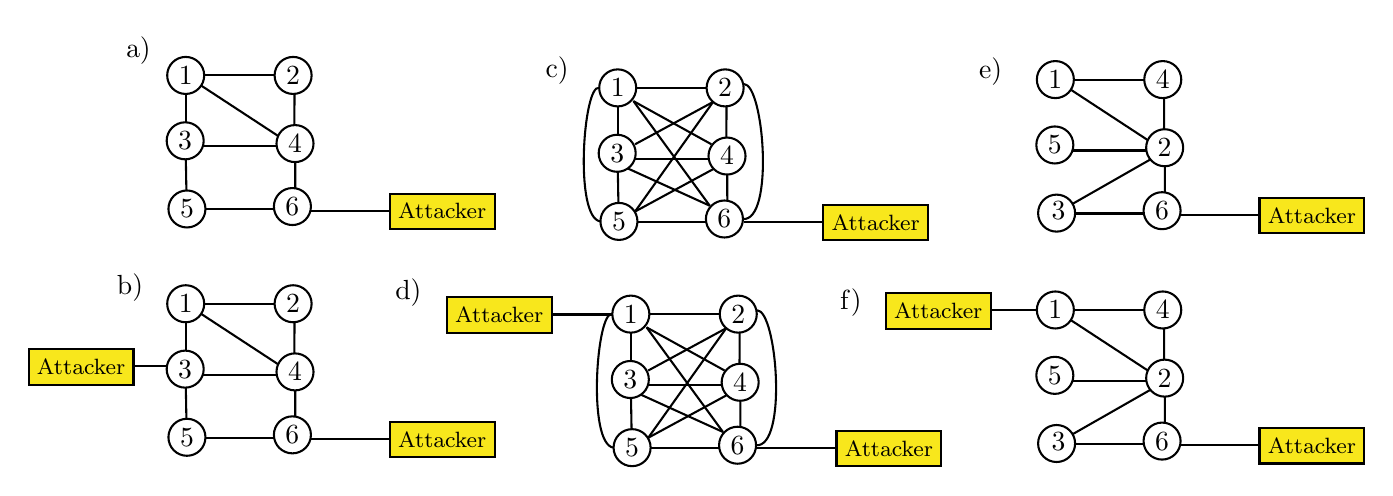
\begin{tikzpicture}[x=0.75pt,y=0.75pt,yscale=-1,xscale=1]
%uncomment if require: \path (0,300); %set diagram left start at 0, and has height of 300

%Straight Lines [id:da21270339539187544] 
\draw    (50.75,166.4) -- (88.67,166.4) ;


%Shape: Rectangle [id:dp19806528063640816] 
\draw  [fill={rgb, 255:red, 248; green, 231; blue, 28 }  ,fill opacity=1 ] (9.2,158.2) -- (59.67,158.2) -- (59.67,175.18) -- (9.2,175.18) -- cycle ;


%Straight Lines [id:da3153834125753151] 
\draw    (137.33,132.22) -- (137.17,163.81) ;


%Straight Lines [id:da7084115546458901] 
\draw    (91.08,200.73) -- (129,200.73) ;


%Straight Lines [id:da9623839826112595] 
\draw    (84.83,136.23) -- (140.58,172.73) ;


%Straight Lines [id:da2909368745777172] 
\draw    (84.83,172.73) -- (85.33,200.55) ;


%Straight Lines [id:da35867881660722734] 
\draw    (137.58,170.73) -- (137.67,202.88) ;


%Shape: Circle [id:dp9939759302306557] 
\draw  [fill={rgb, 255:red, 255; green, 255; blue, 255 }  ,fill opacity=1 ] (75.92,136.23) .. controls (75.92,131.3) and (79.91,127.31) .. (84.83,127.31) .. controls (89.76,127.31) and (93.75,131.3) .. (93.75,136.23) .. controls (93.75,141.15) and (89.76,145.15) .. (84.83,145.15) .. controls (79.91,145.15) and (75.92,141.15) .. (75.92,136.23) -- cycle ;

%Shape: Circle [id:dp34760301125310855] 
\draw  [fill={rgb, 255:red, 255; green, 255; blue, 255 }  ,fill opacity=1 ] (128.58,169.06) .. controls (128.58,164.14) and (132.58,160.15) .. (137.5,160.15) .. controls (142.42,160.15) and (146.42,164.14) .. (146.42,169.06) .. controls (146.42,173.99) and (142.42,177.98) .. (137.5,177.98) .. controls (132.58,177.98) and (128.58,173.99) .. (128.58,169.06) -- cycle ;

%Shape: Circle [id:dp9702116004071654] 
\draw  [fill={rgb, 255:red, 255; green, 255; blue, 255 }  ,fill opacity=1 ] (127.33,199.4) .. controls (127.33,194.47) and (131.33,190.48) .. (136.25,190.48) .. controls (141.17,190.48) and (145.17,194.47) .. (145.17,199.4) .. controls (145.17,204.32) and (141.17,208.31) .. (136.25,208.31) .. controls (131.33,208.31) and (127.33,204.32) .. (127.33,199.4) -- cycle ;

%Straight Lines [id:da8265544446705831] 
\draw    (93.75,136.23) -- (131.67,136.23) ;


%Straight Lines [id:da1435228669726185] 
\draw    (90.75,170.4) -- (128.67,170.4) ;


%Straight Lines [id:da5512583348761163] 
\draw    (84.83,145.15) -- (84.83,163.81) ;


%Shape: Circle [id:dp33954226442737345] 
\draw  [fill={rgb, 255:red, 255; green, 255; blue, 255 }  ,fill opacity=1 ] (76.52,200.56) .. controls (76.52,195.64) and (80.51,191.65) .. (85.43,191.65) .. controls (90.36,191.65) and (94.35,195.64) .. (94.35,200.56) .. controls (94.35,205.49) and (90.36,209.48) .. (85.43,209.48) .. controls (80.51,209.48) and (76.52,205.49) .. (76.52,200.56) -- cycle ;

%Shape: Circle [id:dp027045110799332694] 
\draw  [fill={rgb, 255:red, 255; green, 255; blue, 255 }  ,fill opacity=1 ] (75.67,167.73) .. controls (75.67,162.8) and (79.66,158.81) .. (84.58,158.81) .. controls (89.51,158.81) and (93.5,162.8) .. (93.5,167.73) .. controls (93.5,172.65) and (89.51,176.65) .. (84.58,176.65) .. controls (79.66,176.65) and (75.67,172.65) .. (75.67,167.73) -- cycle ;

%Shape: Circle [id:dp8622510797031577] 
\draw  [fill={rgb, 255:red, 255; green, 255; blue, 255 }  ,fill opacity=1 ] (127.67,136.23) .. controls (127.67,131.3) and (131.66,127.31) .. (136.58,127.31) .. controls (141.51,127.31) and (145.5,131.3) .. (145.5,136.23) .. controls (145.5,141.15) and (141.51,145.15) .. (136.58,145.15) .. controls (131.66,145.15) and (127.67,141.15) .. (127.67,136.23) -- cycle ;

%Straight Lines [id:da8162398929728556] 
\draw    (144.75,201.4) -- (182.67,201.4) ;


%Shape: Rectangle [id:dp15602990655598958] 
\draw  [fill={rgb, 255:red, 248; green, 231; blue, 28 }  ,fill opacity=1 ] (183.2,193.2) -- (233.67,193.2) -- (233.67,210.18) -- (183.2,210.18) -- cycle ;




%Straight Lines [id:da675337569741544] 
\draw    (137.33,22.22) -- (137.17,53.81) ;


%Straight Lines [id:da9770217193149313] 
\draw    (91.08,90.73) -- (129,90.73) ;


%Straight Lines [id:da18857026751215256] 
\draw    (84.83,26.23) -- (140.58,62.73) ;


%Straight Lines [id:da6275844068359788] 
\draw    (84.83,62.73) -- (85.33,90.55) ;


%Straight Lines [id:da3859409733288094] 
\draw    (137.58,60.73) -- (137.67,92.88) ;


%Shape: Circle [id:dp38555186789719464] 
\draw  [fill={rgb, 255:red, 255; green, 255; blue, 255 }  ,fill opacity=1 ] (75.92,26.23) .. controls (75.92,21.3) and (79.91,17.31) .. (84.83,17.31) .. controls (89.76,17.31) and (93.75,21.3) .. (93.75,26.23) .. controls (93.75,31.15) and (89.76,35.15) .. (84.83,35.15) .. controls (79.91,35.15) and (75.92,31.15) .. (75.92,26.23) -- cycle ;

%Shape: Circle [id:dp6614919206504822] 
\draw  [fill={rgb, 255:red, 255; green, 255; blue, 255 }  ,fill opacity=1 ] (128.58,59.06) .. controls (128.58,54.14) and (132.58,50.15) .. (137.5,50.15) .. controls (142.42,50.15) and (146.42,54.14) .. (146.42,59.06) .. controls (146.42,63.99) and (142.42,67.98) .. (137.5,67.98) .. controls (132.58,67.98) and (128.58,63.99) .. (128.58,59.06) -- cycle ;

%Shape: Circle [id:dp4792028510349877] 
\draw  [fill={rgb, 255:red, 255; green, 255; blue, 255 }  ,fill opacity=1 ] (127.33,89.4) .. controls (127.33,84.47) and (131.33,80.48) .. (136.25,80.48) .. controls (141.17,80.48) and (145.17,84.47) .. (145.17,89.4) .. controls (145.17,94.32) and (141.17,98.31) .. (136.25,98.31) .. controls (131.33,98.31) and (127.33,94.32) .. (127.33,89.4) -- cycle ;

%Straight Lines [id:da5503390690988923] 
\draw    (93.75,26.23) -- (131.67,26.23) ;


%Straight Lines [id:da4684291204598492] 
\draw    (90.75,60.4) -- (128.67,60.4) ;


%Straight Lines [id:da14625515615077633] 
\draw    (84.83,35.15) -- (84.83,53.81) ;


%Shape: Circle [id:dp5312971223005962] 
\draw  [fill={rgb, 255:red, 255; green, 255; blue, 255 }  ,fill opacity=1 ] (76.52,90.56) .. controls (76.52,85.64) and (80.51,81.65) .. (85.43,81.65) .. controls (90.36,81.65) and (94.35,85.64) .. (94.35,90.56) .. controls (94.35,95.49) and (90.36,99.48) .. (85.43,99.48) .. controls (80.51,99.48) and (76.52,95.49) .. (76.52,90.56) -- cycle ;

%Shape: Circle [id:dp8123330510491519] 
\draw  [fill={rgb, 255:red, 255; green, 255; blue, 255 }  ,fill opacity=1 ] (75.67,57.73) .. controls (75.67,52.8) and (79.66,48.81) .. (84.58,48.81) .. controls (89.51,48.81) and (93.5,52.8) .. (93.5,57.73) .. controls (93.5,62.65) and (89.51,66.65) .. (84.58,66.65) .. controls (79.66,66.65) and (75.67,62.65) .. (75.67,57.73) -- cycle ;

%Shape: Circle [id:dp008503760549775086] 
\draw  [fill={rgb, 255:red, 255; green, 255; blue, 255 }  ,fill opacity=1 ] (127.67,26.23) .. controls (127.67,21.3) and (131.66,17.31) .. (136.58,17.31) .. controls (141.51,17.31) and (145.5,21.3) .. (145.5,26.23) .. controls (145.5,31.15) and (141.51,35.15) .. (136.58,35.15) .. controls (131.66,35.15) and (127.67,31.15) .. (127.67,26.23) -- cycle ;

%Straight Lines [id:da5256421122460654] 
\draw    (144.75,91.4) -- (182.67,91.4) ;


%Shape: Rectangle [id:dp7797605979818211] 
\draw  [fill={rgb, 255:red, 248; green, 231; blue, 28 }  ,fill opacity=1 ] (183.2,83.2) -- (233.67,83.2) -- (233.67,100.18) -- (183.2,100.18) -- cycle ;




%Straight Lines [id:da22867619419553487] 
\draw    (345.47,28.22) -- (345.31,59.81) ;


%Straight Lines [id:da7366629057200433] 
\draw    (299.22,96.73) -- (337.14,96.73) ;


%Straight Lines [id:da5560609381608291] 
\draw    (292.97,68.73) -- (293.47,96.55) ;


%Straight Lines [id:da4739025620423759] 
\draw    (345.72,66.73) -- (345.81,98.88) ;


%Shape: Circle [id:dp9922005762933758] 
\draw  [fill={rgb, 255:red, 255; green, 255; blue, 255 }  ,fill opacity=1 ] (284.06,32.23) .. controls (284.06,27.3) and (288.05,23.31) .. (292.97,23.31) .. controls (297.9,23.31) and (301.89,27.3) .. (301.89,32.23) .. controls (301.89,37.15) and (297.9,41.15) .. (292.97,41.15) .. controls (288.05,41.15) and (284.06,37.15) .. (284.06,32.23) -- cycle ;

%Shape: Circle [id:dp7388325613342047] 
\draw  [fill={rgb, 255:red, 255; green, 255; blue, 255 }  ,fill opacity=1 ] (336.72,65.06) .. controls (336.72,60.14) and (340.72,56.15) .. (345.64,56.15) .. controls (350.57,56.15) and (354.56,60.14) .. (354.56,65.06) .. controls (354.56,69.99) and (350.57,73.98) .. (345.64,73.98) .. controls (340.72,73.98) and (336.72,69.99) .. (336.72,65.06) -- cycle ;

%Shape: Circle [id:dp3047262312307377] 
\draw  [fill={rgb, 255:red, 255; green, 255; blue, 255 }  ,fill opacity=1 ] (335.47,95.4) .. controls (335.47,90.47) and (339.47,86.48) .. (344.39,86.48) .. controls (349.32,86.48) and (353.31,90.47) .. (353.31,95.4) .. controls (353.31,100.32) and (349.32,104.31) .. (344.39,104.31) .. controls (339.47,104.31) and (335.47,100.32) .. (335.47,95.4) -- cycle ;

%Straight Lines [id:da5232789861595977] 
\draw    (301.89,32.23) -- (339.81,32.23) ;


%Straight Lines [id:da39641445777079876] 
\draw    (298.89,66.4) -- (336.81,66.4) ;


%Straight Lines [id:da6500529894480953] 
\draw    (292.97,41.15) -- (292.97,59.81) ;


%Shape: Circle [id:dp421295758241513] 
\draw  [fill={rgb, 255:red, 255; green, 255; blue, 255 }  ,fill opacity=1 ] (284.66,96.56) .. controls (284.66,91.64) and (288.65,87.65) .. (293.57,87.65) .. controls (298.5,87.65) and (302.49,91.64) .. (302.49,96.56) .. controls (302.49,101.49) and (298.5,105.48) .. (293.57,105.48) .. controls (288.65,105.48) and (284.66,101.49) .. (284.66,96.56) -- cycle ;

%Shape: Circle [id:dp68993621237352] 
\draw  [fill={rgb, 255:red, 255; green, 255; blue, 255 }  ,fill opacity=1 ] (283.81,63.73) .. controls (283.81,58.8) and (287.8,54.81) .. (292.72,54.81) .. controls (297.65,54.81) and (301.64,58.8) .. (301.64,63.73) .. controls (301.64,68.65) and (297.65,72.65) .. (292.72,72.65) .. controls (287.8,72.65) and (283.81,68.65) .. (283.81,63.73) -- cycle ;

%Shape: Circle [id:dp0004348717523896539] 
\draw  [fill={rgb, 255:red, 255; green, 255; blue, 255 }  ,fill opacity=1 ] (335.81,32.23) .. controls (335.81,27.3) and (339.8,23.31) .. (344.72,23.31) .. controls (349.65,23.31) and (353.64,27.3) .. (353.64,32.23) .. controls (353.64,37.15) and (349.65,41.15) .. (344.72,41.15) .. controls (339.8,41.15) and (335.81,37.15) .. (335.81,32.23) -- cycle ;

%Straight Lines [id:da3470843344836425] 
\draw    (297.74,71) -- (337.34,89) ;


%Straight Lines [id:da22385827339648745] 
\draw    (300.54,38.6) -- (338.14,59.4) ;


%Straight Lines [id:da9470627692324495] 
\draw    (301.34,59.4) -- (338.94,39) ;


%Straight Lines [id:da527163614428479] 
\draw    (301.34,91.8) -- (338.94,71.4) ;


%Curve Lines [id:da2659177622157741] 
\draw    (353.81,30.33) .. controls (363.47,30.67) and (368.47,96.67) .. (353.31,95.4) ;


%Curve Lines [id:da3968887523398855] 
\draw    (284.06,32.23) .. controls (276.47,30) and (271.81,95) .. (284.66,96.56) ;


%Straight Lines [id:da4862470624661749] 
\draw    (300.54,38.6) -- (337.34,89) ;


%Straight Lines [id:da9265421066580971] 
\draw    (338.94,39) -- (301.34,91.8) ;


%Straight Lines [id:da7131649869831252] 
\draw    (353.61,96.82) -- (391.52,96.82) ;


%Shape: Rectangle [id:dp3615803597823173] 
\draw  [fill={rgb, 255:red, 248; green, 231; blue, 28 }  ,fill opacity=1 ] (392.06,88.63) -- (442.53,88.63) -- (442.53,105.61) -- (392.06,105.61) -- cycle ;




%Straight Lines [id:da6715977826012206] 
\draw    (351.81,137.22) -- (351.64,168.81) ;


%Straight Lines [id:da9540657786576023] 
\draw    (305.56,205.73) -- (343.48,205.73) ;


%Straight Lines [id:da5731952874596753] 
\draw    (299.31,177.73) -- (299.81,205.55) ;


%Straight Lines [id:da41041637205710924] 
\draw    (352.06,175.73) -- (352.14,207.88) ;


%Shape: Circle [id:dp7490995910930758] 
\draw  [fill={rgb, 255:red, 255; green, 255; blue, 255 }  ,fill opacity=1 ] (290.39,141.23) .. controls (290.39,136.3) and (294.38,132.31) .. (299.31,132.31) .. controls (304.23,132.31) and (308.23,136.3) .. (308.23,141.23) .. controls (308.23,146.15) and (304.23,150.15) .. (299.31,150.15) .. controls (294.38,150.15) and (290.39,146.15) .. (290.39,141.23) -- cycle ;

%Shape: Circle [id:dp21867347242120194] 
\draw  [fill={rgb, 255:red, 255; green, 255; blue, 255 }  ,fill opacity=1 ] (343.06,174.06) .. controls (343.06,169.14) and (347.05,165.15) .. (351.98,165.15) .. controls (356.9,165.15) and (360.89,169.14) .. (360.89,174.06) .. controls (360.89,178.99) and (356.9,182.98) .. (351.98,182.98) .. controls (347.05,182.98) and (343.06,178.99) .. (343.06,174.06) -- cycle ;

%Shape: Circle [id:dp009688206133991684] 
\draw  [fill={rgb, 255:red, 255; green, 255; blue, 255 }  ,fill opacity=1 ] (341.81,204.4) .. controls (341.81,199.47) and (345.8,195.48) .. (350.73,195.48) .. controls (355.65,195.48) and (359.64,199.47) .. (359.64,204.4) .. controls (359.64,209.32) and (355.65,213.31) .. (350.73,213.31) .. controls (345.8,213.31) and (341.81,209.32) .. (341.81,204.4) -- cycle ;

%Straight Lines [id:da45622560516359056] 
\draw    (308.23,141.23) -- (346.14,141.23) ;


%Straight Lines [id:da8381919416870578] 
\draw    (305.23,175.4) -- (343.14,175.4) ;


%Straight Lines [id:da6163529535308253] 
\draw    (299.31,150.15) -- (299.31,168.81) ;


%Shape: Circle [id:dp456728946120202] 
\draw  [fill={rgb, 255:red, 255; green, 255; blue, 255 }  ,fill opacity=1 ] (290.99,205.56) .. controls (290.99,200.64) and (294.98,196.65) .. (299.91,196.65) .. controls (304.83,196.65) and (308.83,200.64) .. (308.83,205.56) .. controls (308.83,210.49) and (304.83,214.48) .. (299.91,214.48) .. controls (294.98,214.48) and (290.99,210.49) .. (290.99,205.56) -- cycle ;

%Shape: Circle [id:dp45682398029629745] 
\draw  [fill={rgb, 255:red, 255; green, 255; blue, 255 }  ,fill opacity=1 ] (290.14,172.73) .. controls (290.14,167.8) and (294.13,163.81) .. (299.06,163.81) .. controls (303.98,163.81) and (307.98,167.8) .. (307.98,172.73) .. controls (307.98,177.65) and (303.98,181.65) .. (299.06,181.65) .. controls (294.13,181.65) and (290.14,177.65) .. (290.14,172.73) -- cycle ;

%Shape: Circle [id:dp20828836021634367] 
\draw  [fill={rgb, 255:red, 255; green, 255; blue, 255 }  ,fill opacity=1 ] (342.14,141.23) .. controls (342.14,136.3) and (346.13,132.31) .. (351.06,132.31) .. controls (355.98,132.31) and (359.98,136.3) .. (359.98,141.23) .. controls (359.98,146.15) and (355.98,150.15) .. (351.06,150.15) .. controls (346.13,150.15) and (342.14,146.15) .. (342.14,141.23) -- cycle ;

%Straight Lines [id:da32117265204513157] 
\draw    (304.08,180) -- (343.68,198) ;


%Straight Lines [id:da6079841314173954] 
\draw    (306.88,147.6) -- (344.48,168.4) ;


%Straight Lines [id:da7680118845457601] 
\draw    (307.68,168.4) -- (345.28,148) ;


%Straight Lines [id:da6389773826545454] 
\draw    (307.68,200.8) -- (345.28,180.4) ;


%Curve Lines [id:da511824766847756] 
\draw    (360.14,139.33) .. controls (369.81,139.67) and (374.81,205.67) .. (359.64,204.4) ;


%Curve Lines [id:da10840460492754567] 
\draw    (290.39,141.23) .. controls (282.81,139) and (278.14,204) .. (290.99,205.56) ;


%Straight Lines [id:da3147720372519749] 
\draw    (306.88,147.6) -- (343.68,198) ;


%Straight Lines [id:da9757233447370841] 
\draw    (345.28,148) -- (307.68,200.8) ;


%Straight Lines [id:da8351826345519837] 
\draw    (359.94,205.82) -- (397.86,205.82) ;


%Shape: Rectangle [id:dp9492523154356004] 
\draw  [fill={rgb, 255:red, 248; green, 231; blue, 28 }  ,fill opacity=1 ] (398.39,197.63) -- (448.86,197.63) -- (448.86,214.61) -- (398.39,214.61) -- cycle ;


%Straight Lines [id:da7783875840754805] 
\draw    (252.23,141.4) -- (290.14,141.4) ;


%Shape: Rectangle [id:dp8219665960733671] 
\draw  [fill={rgb, 255:red, 248; green, 231; blue, 28 }  ,fill opacity=1 ] (210.68,133.2) -- (261.15,133.2) -- (261.15,150.18) -- (210.68,150.18) -- cycle ;



%Straight Lines [id:da7147269629924605] 
\draw    (556.33,24.22) -- (556.17,55.81) ;


%Straight Lines [id:da8277651830187894] 
\draw    (510.08,92.73) -- (548,92.73) ;


%Straight Lines [id:da0013601110130750937] 
\draw    (503.83,28.23) -- (559.58,64.73) ;


%Straight Lines [id:da5364857137309426] 
\draw    (556.58,62.73) -- (504.33,92.55) ;


%Straight Lines [id:da09227991689524317] 
\draw    (556.58,62.73) -- (556.67,94.88) ;


%Shape: Circle [id:dp40945899905332894] 
\draw  [fill={rgb, 255:red, 255; green, 255; blue, 255 }  ,fill opacity=1 ] (494.92,28.23) .. controls (494.92,23.3) and (498.91,19.31) .. (503.83,19.31) .. controls (508.76,19.31) and (512.75,23.3) .. (512.75,28.23) .. controls (512.75,33.15) and (508.76,37.15) .. (503.83,37.15) .. controls (498.91,37.15) and (494.92,33.15) .. (494.92,28.23) -- cycle ;

%Shape: Circle [id:dp7767184939243962] 
\draw  [fill={rgb, 255:red, 255; green, 255; blue, 255 }  ,fill opacity=1 ] (547.58,61.06) .. controls (547.58,56.14) and (551.58,52.15) .. (556.5,52.15) .. controls (561.42,52.15) and (565.42,56.14) .. (565.42,61.06) .. controls (565.42,65.99) and (561.42,69.98) .. (556.5,69.98) .. controls (551.58,69.98) and (547.58,65.99) .. (547.58,61.06) -- cycle ;
%Shape: Circle [id:dp4692699516703288] 
\draw  [fill={rgb, 255:red, 255; green, 255; blue, 255 }  ,fill opacity=1 ] (546.33,91.4) .. controls (546.33,86.47) and (550.33,82.48) .. (555.25,82.48) .. controls (560.17,82.48) and (564.17,86.47) .. (564.17,91.4) .. controls (564.17,96.32) and (560.17,100.31) .. (555.25,100.31) .. controls (550.33,100.31) and (546.33,96.32) .. (546.33,91.4) -- cycle ;

%Straight Lines [id:da9597316941694047] 
\draw    (512.75,28.23) -- (550.67,28.23) ;


%Straight Lines [id:da7708545450116795] 
\draw    (509.75,62.4) -- (547.67,62.4) ;


%Shape: Circle [id:dp40660215241265885] 
\draw  [fill={rgb, 255:red, 255; green, 255; blue, 255 }  ,fill opacity=1 ] (495.52,92.56) .. controls (495.52,87.64) and (499.51,83.65) .. (504.43,83.65) .. controls (509.36,83.65) and (513.35,87.64) .. (513.35,92.56) .. controls (513.35,97.49) and (509.36,101.48) .. (504.43,101.48) .. controls (499.51,101.48) and (495.52,97.49) .. (495.52,92.56) -- cycle ;
%Shape: Circle [id:dp09457558597010363] 
\draw  [fill={rgb, 255:red, 255; green, 255; blue, 255 }  ,fill opacity=1 ] (494.67,59.73) .. controls (494.67,54.8) and (498.66,50.81) .. (503.58,50.81) .. controls (508.51,50.81) and (512.5,54.8) .. (512.5,59.73) .. controls (512.5,64.65) and (508.51,68.65) .. (503.58,68.65) .. controls (498.66,68.65) and (494.67,64.65) .. (494.67,59.73) -- cycle ;
%Shape: Circle [id:dp7445040256787864] 
\draw  [fill={rgb, 255:red, 255; green, 255; blue, 255 }  ,fill opacity=1 ] (546.67,28.23) .. controls (546.67,23.3) and (550.66,19.31) .. (555.58,19.31) .. controls (560.51,19.31) and (564.5,23.3) .. (564.5,28.23) .. controls (564.5,33.15) and (560.51,37.15) .. (555.58,37.15) .. controls (550.66,37.15) and (546.67,33.15) .. (546.67,28.23) -- cycle ;
%Straight Lines [id:da6980179493369204] 
\draw    (563.75,93.4) -- (601.67,93.4) ;


%Shape: Rectangle [id:dp9981691173299058] 
\draw  [fill={rgb, 255:red, 248; green, 231; blue, 28 }  ,fill opacity=1 ] (602.2,85.2) -- (652.67,85.2) -- (652.67,102.18) -- (602.2,102.18) -- cycle ;




%Straight Lines [id:da8092387671610324] 
\draw    (463.75,139.4) -- (501.67,139.4) ;


%Shape: Rectangle [id:dp7958055249044546] 
\draw  [fill={rgb, 255:red, 248; green, 231; blue, 28 }  ,fill opacity=1 ] (422.2,131.2) -- (472.67,131.2) -- (472.67,148.18) -- (422.2,148.18) -- cycle ;


%Straight Lines [id:da8513354272469744] 
\draw    (556.33,135.22) -- (556.17,166.81) ;


%Straight Lines [id:da7992137672953211] 
\draw    (510.08,203.73) -- (548,203.73) ;


%Straight Lines [id:da3954660742507915] 
\draw    (503.83,139.23) -- (559.58,175.73) ;


%Straight Lines [id:da5825560768425334] 
\draw    (556.58,173.73) -- (504.33,203.55) ;


%Straight Lines [id:da5568053188323774] 
\draw    (556.58,173.73) -- (556.67,205.88) ;


%Shape: Circle [id:dp30253748945575554] 
\draw  [fill={rgb, 255:red, 255; green, 255; blue, 255 }  ,fill opacity=1 ] (494.92,139.23) .. controls (494.92,134.3) and (498.91,130.31) .. (503.83,130.31) .. controls (508.76,130.31) and (512.75,134.3) .. (512.75,139.23) .. controls (512.75,144.15) and (508.76,148.15) .. (503.83,148.15) .. controls (498.91,148.15) and (494.92,144.15) .. (494.92,139.23) -- cycle ;

%Shape: Circle [id:dp3641428183407782] 
\draw  [fill={rgb, 255:red, 255; green, 255; blue, 255 }  ,fill opacity=1 ] (547.58,172.06) .. controls (547.58,167.14) and (551.58,163.15) .. (556.5,163.15) .. controls (561.42,163.15) and (565.42,167.14) .. (565.42,172.06) .. controls (565.42,176.99) and (561.42,180.98) .. (556.5,180.98) .. controls (551.58,180.98) and (547.58,176.99) .. (547.58,172.06) -- cycle ;
%Shape: Circle [id:dp08738614749957285] 
\draw  [fill={rgb, 255:red, 255; green, 255; blue, 255 }  ,fill opacity=1 ] (546.33,202.4) .. controls (546.33,197.47) and (550.33,193.48) .. (555.25,193.48) .. controls (560.17,193.48) and (564.17,197.47) .. (564.17,202.4) .. controls (564.17,207.32) and (560.17,211.31) .. (555.25,211.31) .. controls (550.33,211.31) and (546.33,207.32) .. (546.33,202.4) -- cycle ;

%Straight Lines [id:da8382293979078496] 
\draw    (512.75,139.23) -- (550.67,139.23) ;


%Straight Lines [id:da06888701209203096] 
\draw    (509.75,173.4) -- (547.67,173.4) ;


%Shape: Circle [id:dp03475136247746857] 
\draw  [fill={rgb, 255:red, 255; green, 255; blue, 255 }  ,fill opacity=1 ] (495.52,203.56) .. controls (495.52,198.64) and (499.51,194.65) .. (504.43,194.65) .. controls (509.36,194.65) and (513.35,198.64) .. (513.35,203.56) .. controls (513.35,208.49) and (509.36,212.48) .. (504.43,212.48) .. controls (499.51,212.48) and (495.52,208.49) .. (495.52,203.56) -- cycle ;
%Shape: Circle [id:dp825936328113765] 
\draw  [fill={rgb, 255:red, 255; green, 255; blue, 255 }  ,fill opacity=1 ] (494.67,170.73) .. controls (494.67,165.8) and (498.66,161.81) .. (503.58,161.81) .. controls (508.51,161.81) and (512.5,165.8) .. (512.5,170.73) .. controls (512.5,175.65) and (508.51,179.65) .. (503.58,179.65) .. controls (498.66,179.65) and (494.67,175.65) .. (494.67,170.73) -- cycle ;
%Shape: Circle [id:dp10791744420385518] 
\draw  [fill={rgb, 255:red, 255; green, 255; blue, 255 }  ,fill opacity=1 ] (546.67,139.23) .. controls (546.67,134.3) and (550.66,130.31) .. (555.58,130.31) .. controls (560.51,130.31) and (564.5,134.3) .. (564.5,139.23) .. controls (564.5,144.15) and (560.51,148.15) .. (555.58,148.15) .. controls (550.66,148.15) and (546.67,144.15) .. (546.67,139.23) -- cycle ;
%Straight Lines [id:da35173459455787404] 
\draw    (563.75,204.4) -- (601.67,204.4) ;


%Shape: Rectangle [id:dp6910000106247179] 
\draw  [fill={rgb, 255:red, 248; green, 231; blue, 28 }  ,fill opacity=1 ] (602.2,196.2) -- (652.67,196.2) -- (652.67,213.18) -- (602.2,213.18) -- cycle ;




% Text Node
\draw (405.33,135.67) node  [align=left] {f)};
% Text Node
\draw (556.5,172.06) node  [align=left] {2};
% Text Node
\draw (505.43,202.56) node  [align=left] {3};
% Text Node
\draw (503.58,170.73) node  [align=left] {5};
% Text Node
\draw (555.58,139.23) node  [align=left] {4};
% Text Node
\draw (627.44,204.69) node  [align=left] {{\footnotesize Attacker}};
% Text Node
\draw (555.25,202.4) node  [align=left] {6};
% Text Node
\draw (503.83,139.23) node  [align=left] {1};
% Text Node
\draw (447.44,139.69) node  [align=left] {{\footnotesize Attacker}};
% Text Node
\draw (472.67,24.33) node  [align=left] {e)};
% Text Node
\draw (556.5,61.06) node  [align=left] {2};
% Text Node
\draw (505.43,91.56) node  [align=left] {3};
% Text Node
\draw (503.58,59.73) node  [align=left] {5};
% Text Node
\draw (555.58,28.23) node  [align=left] {4};
% Text Node
\draw (627.44,93.69) node  [align=left] {{\footnotesize Attacker}};
% Text Node
\draw (555.25,91.4) node  [align=left] {6};
% Text Node
\draw (503.83,28.23) node  [align=left] {1};
% Text Node
\draw (192.14,131) node  [align=left] {d)};
% Text Node
\draw (235.91,141.69) node  [align=left] {{\footnotesize Attacker}};
% Text Node
\draw (423.63,206.12) node  [align=left] {{\footnotesize Attacker}};
% Text Node
\draw (351.06,141.23) node  [align=left] {2};
% Text Node
\draw (299.06,172.73) node  [align=left] {3};
% Text Node
\draw (299.91,205.56) node  [align=left] {5};
% Text Node
\draw (350.73,204.4) node  [align=left] {6};
% Text Node
\draw (351.98,174.06) node  [align=left] {4};
% Text Node
\draw (299.31,141.23) node  [align=left] {1};
% Text Node
\draw (263.81,24) node  [align=left] {c)};
% Text Node
\draw (417.29,97.12) node  [align=left] {{\footnotesize Attacker}};
% Text Node
\draw (344.72,32.23) node  [align=left] {2};
% Text Node
\draw (292.72,63.73) node  [align=left] {3};
% Text Node
\draw (293.57,96.56) node  [align=left] {5};
% Text Node
\draw (344.39,95.4) node  [align=left] {6};
% Text Node
\draw (345.64,65.06) node  [align=left] {4};
% Text Node
\draw (292.97,32.23) node  [align=left] {1};
% Text Node
\draw (62,14.33) node  [align=left] {a)};
% Text Node
\draw (208.44,91.69) node  [align=left] {{\footnotesize Attacker}};
% Text Node
\draw (136.58,26.23) node  [align=left] {2};
% Text Node
\draw (84.58,57.73) node  [align=left] {3};
% Text Node
\draw (85.43,90.56) node  [align=left] {5};
% Text Node
\draw (136.25,89.4) node  [align=left] {6};
% Text Node
\draw (137.5,59.06) node  [align=left] {4};
% Text Node
\draw (84.83,26.23) node  [align=left] {1};
% Text Node
\draw (58,128.33) node  [align=left] {b)};
% Text Node
\draw (208.44,201.69) node  [align=left] {{\footnotesize Attacker}};
% Text Node
\draw (136.58,136.23) node  [align=left] {2};
% Text Node
\draw (84.58,167.73) node  [align=left] {3};
% Text Node
\draw (85.43,200.56) node  [align=left] {5};
% Text Node
\draw (136.25,199.4) node  [align=left] {6};
% Text Node
\draw (137.5,169.06) node  [align=left] {4};
% Text Node
\draw (84.83,136.23) node  [align=left] {1};
% Text Node
\draw (34.44,166.69) node  [align=left] {{\footnotesize Attacker}};


\end{tikzpicture}


\caption{Use case topologies}
\label{fig:mdp-usecase-single}
\end{figure}

We run the MDP using different budgets and detection probabilities.
Nodes are migrated in the following order: 1, 2 and 3.
The ordering of the nodes impacts the result sets of Algorithm~\ref{algo:target}, thus which nodes may be attacked at each transition.
We have extracted the monitoring set of each absorbing state, and evaluated the overall reward of each monitoring set.
We define the reward of a monitoring set as the expected value of the reward of each corresponding absorbing state.
The expected value uses the stationary distribution of the Markov Chain corresponding to the optimal policy.
Details about the source node for attacks again the migration is summarized in Table~\ref{tab:mdp-attack-source}.

% Please add the following required packages to your document preamble:
% \usepackage{graphicx}
\begin{table}[h]
\resizebox{\textwidth}{!}{%
\begin{tabular}{|c|c|c|c|c|c|c|c|c|c|c|c|c|c|c|c|c|c|c|c|c|c|c|}
\cline{1-7} \cline{9-15} \cline{17-23}
\multicolumn{7}{|c|}{\textbf{Scenario b)}} &  & \multicolumn{7}{c|}{\textbf{Scenario d)}} &  & \multicolumn{7}{c|}{\textbf{Scenario f)}} \\ \cline{1-7} \cline{9-15} \cline{17-23} 
Target node    & 1  & 2  & 3  & 4  & 5 & 6 &  & Target node    & 1  & 2  & 3  & 4 & 5 & 6 &  & Target node    & 1  & 2  & 3  & 4 & 5 & 6 \\ \cline{1-7} \cline{9-15} \cline{17-23} 
Attack source  & 6  & 4  & 6  & 4  & 6 & 6 &  & Attack Source  & 6  & 6  & 1  & 6 & 1 & 1 &  & Attack source  & 6  & 6  & 1  & 6 & 1 & 1 \\ \cline{1-7} \cline{9-15} \cline{17-23} 
\end{tabular}%
}
\caption{Attack sources for multiple attackers scenarios}
\label{tab:mdp-attack-source}
\end{table}

\textbf{Scenario a) and b)\\}
Based on the paths taken by attacks and the ordering of the migration, we categorize the nodes into three categories: source, intermediate and border nodes. Source nodes are the origins of attacks, intermediate nodes are going to be on the path of attacks targeting the border nodes. 
The results are shown in Fig.~\ref{fig:mdp-result-topo1}.
The scenario a) sets the source to node 6, nodes 4 and 5 as intermediate nodes and finally nodes 1,2 and 3 as border nodes.
The scenario b) sets the source to nodes 3 and 6, nodes 1,4 as intermediate and nodes 2 and 5 as border nodes.
The first observation is that node 6 is globally the most rewarding node in both cases.
This is explained as it is the source of most of the attacks, and the exfiltrated data is redirected there.
In both scenarios the importance of nodes is separated according to the our categorization. 
This means that the nodes pertaining to the majority of attack paths are the most rewarded.
This is observation is reinforced in scenario b) where nodes 4 and 5 are close to attack sources while nodes 1 and 2 are further away.

In both scenarios, the detection rate does not have a significant impact on the ranking of the nodes, compared to each other.
In scenario a) results are stable from $p=0.6$ where node 6 overcomes node 4 in reward until $p=0.9$. All other nodes remain closely grouped, and no intermediate or border nodes is standing out.
In scenario b) the higher the detection rate the higher the reward of node 3, the second source of attacks.
The steadiness in the evolution of each node shows that the performance of the detection is not a major factor in determining which nodes are best suited for the monitoring. We formulate some hypotheses in Section~\ref{sec:mdp-discussion}.

Detailed examination of the optimal policy for each budget also shows that the monitoring action is rarely used to redeploy resource elsewhere in the infrastructure.
Instead of unmonitoring nodes, the MDP chooses to do nothing to preserve the global detection probability.
$m_j$ actions are only chosen when the unmonitored node does not detect the next attack, thus having the same impact as action $d$. These corner cases only represent a small percentage of the global solution where very few attacks occurred.

\textbf{Scenarios c) and d) \\}
In these scenarios, the topology considered is fullmeshed, which means that each physical node is connected to every other node of the infrastructure. This topology has been chosen to minimize the impact of the routing on the detection path because the attacker is always connected to the target node.
Results are shown in Fig.~\ref{fig:mdp-result-fullmesh}.

The first observation we make is that whether there is one or several attackers, the position of nodes between each other remains unchanged. This reinforce our conclusion that the routing of attacks has a real impact on the detection performance of each node.
The second observation we make is that the most important nodes are the main source of attacks as well as the first node being migrated. While the first node is an obvious choice for attack detection, the second shows another aspect of the model which is target selection. Indeed, since node 1 is always migrated first, it is therefore the main target at the first transition of the MDP.

% Finally, we have examined the different optimal policies for these scenarios, and observed that some corner cases have appeared.
Overall, the fact that for each attack only the origin of the attack and the target node may contribute to the detection has generated a diverse solution state. Indeed, depending on which node would be targeted there is a unique solution set to detect the attack and the fullmesh aspect of the topology makes it hard for those solution sets to overlap and give a better coverage.

\textbf{Scenarios e) and f) \\}

Using the same categorization as scenarios a) and b), we consider node 6 as a source node, node 2 as an intermediate node and nodes 1,3,4,5 as border nodes. Scenario f) transfers node 1 from a border node to a source node. Results are shown in Fig.~\ref{fig:mdp-result-topo2}.

In scenario e), the importance of each node depicted in Fig.~\ref{fig:mdp-result-topo2} reflect their role. Nodes 1,3,4 and 5 do not have much impact in the solution set, as they are not on the path of most of attacks. The attack source is still considered important to monitor and node 2 which acts as a ``bridge" between the two halves of the topology will belong to the path of a lot of attacks.

Scenario f) highlights similar results. There are now two attack sources, nodes 1 and 6. Moreover, the geographical distribution of migrated nodes gives more importance to node 2 which becomes even more present on the attack paths, as shown in Table~\ref{tab:mdp-attack-source}. This scenario is also the only one in which the main source of attacks is not consistently the most important node for the monitoring.

% Optimal policies also have some corner cases with counter intuitive optimal monitoring nodes but those remain marginal considering the solution space. 



\begin{figure}
    \centering
    \captionsetup[subfigure]{labelformat=empty}
\begin{subfigure}{.5\textwidth}
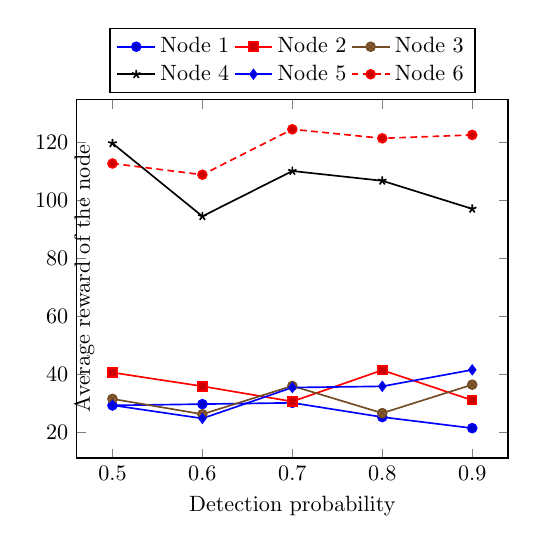
\begin{tikzpicture}[scale=0.8]
\begin{axis}[
  xlabel={Detection probability},
  ylabel={Average reward of the node },
  y label style={at={(0.06,0.5)}},
  xtick={0.5,0.6,0.7,0.8,0.9,1.0},
  legend style={at={(0.5,1.2)},cells={align=right}, anchor=north,legend columns=3},
  grid style=dashed,
]

\addplot+[]
    coordinates {
(0.5,29.2207587022)(0.6,29.6591500811)(0.7,30.107769581)(0.8,25.1808225374)(0.9,21.3501334315)
};

\addplot+[]
    coordinates {
(0.5,40.5649596864)(0.6,35.8317201966)(0.7,30.5615817425)(0.8,41.4017616625)(0.9,31.0018428294)
};

\addplot+[]
    coordinates {
(0.5,31.4601711216)(0.6,26.1715912622)(0.7,35.9427616495)(0.8,26.5488358659)(0.9,36.3780765072)
};

\addplot+[]
    coordinates {
(0.5,119.788927983)(0.6,94.566243579)(0.7,110.212449824)(0.8,106.844518821)(0.9,97.138069126)
};

\addplot+[]
    coordinates {
(0.5,29.2697135288)(0.6,24.7098561839)(0.7,35.3909999115)(0.8,35.8083893589)(0.9,41.5087141375)
};

\addplot+[]
    coordinates {
(0.5,112.808511307)(0.6,108.932780706)(0.7,124.631408718)(0.8,121.507931814)(0.9,122.678991306)
};

\legend{Node 1, Node 2, Node 3, Node 4, Node 5, Node 6}
\end{axis}
\end{tikzpicture}

\caption{Scenario a)}
\label{fig:nodeimp_single}
\end{subfigure}
\begin{subfigure}{.33\textwidth}
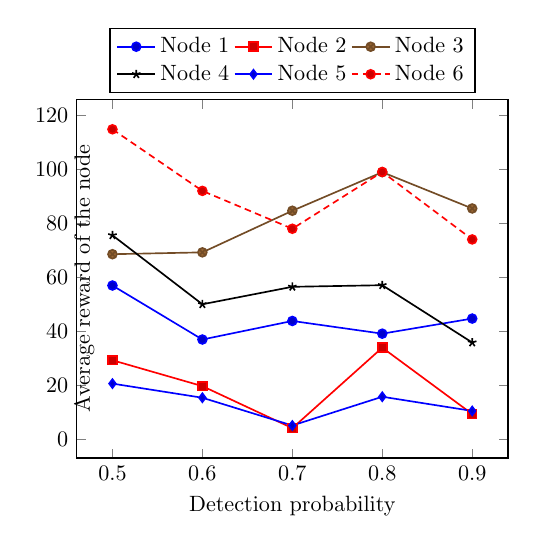
\begin{tikzpicture}[scale=0.8]
\begin{axis}[
  xlabel={Detection probability},
  ylabel={Average reward of the node },
  y label style={at={(0.06,0.5)}},
  xtick={0.5,0.6,0.7,0.8,0.9,1.0},
  legend style={at={(0.5,1.2)},cells={align=right}, anchor=north,legend columns=3},
  grid style=dashed,
]

\addplot+[]
    coordinates {
(0.5,57.0711574474)(0.6,37.0782125822)(0.7,43.9471043804)(0.8,39.2446371458)(0.9,44.8363801675)
};

\addplot+[]
    coordinates {
(0.5,29.4097815394)(0.6,19.8278112984)(0.7,4.26428571429)(0.8,34.0706693208)(0.9,9.49928571429)
};

\addplot+[]
    coordinates {
(0.5,68.6596096998)(0.6,69.339332514)(0.7,84.7438538657)(0.8,99.0264041517)(0.9,85.5894326243)
};

\addplot+[]
    coordinates {
(0.5,75.6609039908)(0.6,50.1243516403)(0.7,56.5923700845)(0.8,57.1874277411)(0.9,35.9649500717)
};

\addplot+[]
    coordinates {
(0.5,20.7573450249)(0.6,15.5267400966)(0.7,5.25375523139)(0.8,15.8992854434)(0.9,10.6415647894)
};

\addplot+[]
    coordinates {
(0.5,114.89762846)(0.6,92.0949728442)(0.7,78.0795310037)(0.8,99.102629324)(0.9,74.1266846482)
};

\legend{Node 1, Node 2, Node 3, Node 4, Node 5, Node 6}
\end{axis}
\end{tikzpicture}

\caption{Scenario b)}
\label{fig:nodeimp_topo1_multiple}
\end{subfigure}
    \caption{Results for single and multiple attackers}
    \label{fig:mdp-result-topo1}
\end{figure}
\begin{figure}
    \centering
    \captionsetup[subfigure]{labelformat=empty}
\begin{subfigure}{.5\textwidth}
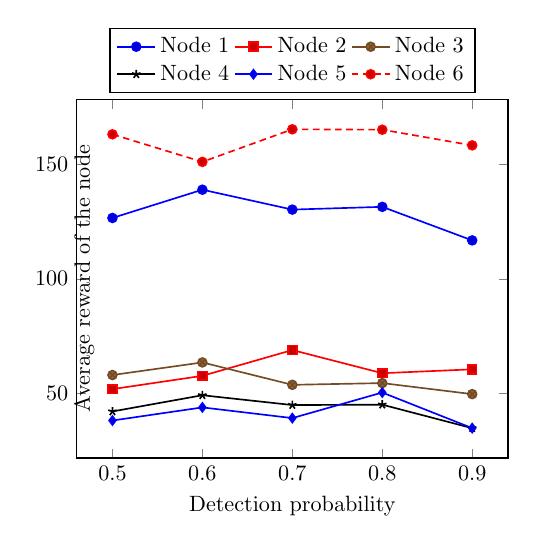
\begin{tikzpicture}[scale=0.8]
\begin{axis}[
  xlabel={Detection probability},
  ylabel={Average reward of the node },
  y label style={at={(0.06,0.5)}},
  xtick={0.5,0.6,0.7,0.8,0.9,1.0},
  legend style={at={(0.5,1.2)},cells={align=right}, anchor=north,legend columns=3},
  grid style=dashed,
]

\addplot+[]
    coordinates {
(0.5,126.469294224)(0.6,138.768688772)(0.7,130.10979383)(0.8,131.308647284)(0.9,116.70873472)
};

\addplot+[]
    coordinates {
(0.5,51.9774584454)(0.6,57.7615872131)(0.7,68.9811633084)(0.8,58.9060250618)(0.9,60.5911805552)
};

\addplot+[]
    coordinates {
(0.5,58.112876005)(0.6,63.5894390224)(0.7,53.8483204974)(0.8,54.5969922461)(0.9,49.8027670671)
};

\addplot+[]
    coordinates {
(0.5,42.2594496478)(0.6,49.3133895991)(0.7,45.0502147208)(0.8,45.20918204)(0.9,34.9808016775)
};

\addplot+[]
    coordinates {
(0.5,38.3055097066)(0.6,44.0188235767)(0.7,39.3680288222)(0.8,50.4912779668)(0.9,34.9978557067)
};

\addplot+[]
    coordinates {
(0.5,162.87848727)(0.6,150.876767477)(0.7,165.06110317)(0.8,164.882126918)(0.9,158.067481047)
};

\legend{Node 1, Node 2, Node 3, Node 4, Node 5, Node 6}
\end{axis}
\end{tikzpicture}

\caption{Scenario c)}
\label{fig:nodeimp_topofullmesh_single}
\end{subfigure}
\begin{subfigure}{.33\textwidth}
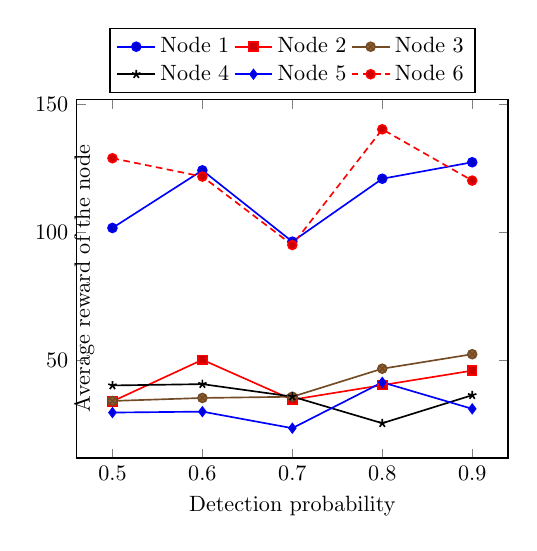
\begin{tikzpicture}[scale=0.8]
\begin{axis}[
  xlabel={Detection probability},
  ylabel={Average reward of the node },
  y label style={at={(0.06,0.5)}},
  xtick={0.5,0.6,0.7,0.8,0.9,1.0},
  legend style={at={(0.5,1.2)},cells={align=right}, anchor=north,legend columns=3},
  grid style=dashed,
]
\addplot+[]
    coordinates {
(0.5,101.616873023)(0.6,124.145242333)(0.7,96.2616914651)(0.8,120.862819291)(0.9,127.305784272)
};

\addplot+[]
    coordinates {
(0.5,33.8037034841)(0.6,50.0693289402)(0.7,34.460597311)(0.8,40.1535742549)(0.9,45.8166364524)
};

\addplot+[]
    coordinates {
(0.5,33.9581528218)(0.6,35.1326808601)(0.7,35.6074089582)(0.8,46.5769811834)(0.9,52.2400544067)
};

\addplot+[]
    coordinates {
(0.5,40.0224063598)(0.6,40.5434953331)(0.7,35.6681036149)(0.8,25.2556265302)(0.9,36.2111392677)
};

\addplot+[]
    coordinates {
(0.5,29.4251886633)(0.6,29.7859232959)(0.7,23.3183642626)(0.8,41.2471235042)(0.9,30.8838558151)
};

\addplot+[]
    coordinates {
(0.5,128.882560148)(0.6,121.704109507)(0.7,94.9489538016)(0.8,140.19719198)(0.9,120.142225907)
};


\legend{Node 1, Node 2, Node 3, Node 4, Node 5, Node 6}
\end{axis}
\end{tikzpicture}

\caption{Scenario d)}
\label{fig:nodeimp_topofullmesh_multiple}
\end{subfigure}
\caption{Results for single and multiple attackers - Scenarios c) and d)}
    \label{fig:mdp-result-fullmesh}
\end{figure}
\begin{figure}
    \centering
    \captionsetup[subfigure]{labelformat=empty}
\begin{subfigure}{.5\textwidth}
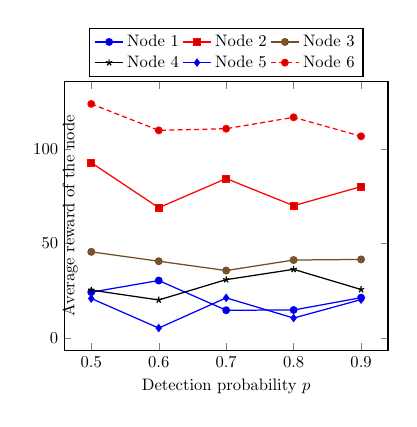
\begin{tikzpicture}[scale=0.6]
\begin{axis}[
  xlabel={Detection probability $p$},
  ylabel={Average reward of the node },
  y label style={at={(0.06,0.5)}},
  xtick={0.5,0.6,0.7,0.8,0.9,1.0},
  legend style={at={(0.5,1.2)},cells={align=right}, anchor=north,legend columns=3},
  grid style=dashed,
]
\addplot+[]
    coordinates {
(0.5,24.2596903238)(0.6,30.4098004181)(0.7,14.7157392372)(0.8,14.8410159329)(0.9,21.3512325325)
};

\addplot+[]
    coordinates {
(0.5,92.6967638225)(0.6,68.892572501)(0.7,84.3050837463)(0.8,69.9668923619)(0.9,80.051680541)
};

\addplot+[]
    coordinates {
(0.5,45.5695982478)(0.6,40.6246377658)(0.7,35.692885081)(0.8,41.2436256503)(0.9,41.5670235599)
};

\addplot+[]
    coordinates {
(0.5,25.3670893308)(0.6,20.1438895136)(0.7,30.888009803)(0.8,36.3312849347)(0.9,25.6728772368)
};

\addplot+[]
    coordinates {
(0.5,20.9174008986)(0.6,5.30161144168)(0.7,21.2602459651)(0.8,10.5837610733)(0.9,20.3331330431)
};

\addplot+[]
    coordinates {
(0.5,123.776293271)(0.6,109.788318837)(0.7,110.653974948)(0.8,116.685625909)(0.9,106.649803871)
};

\legend{Node 1, Node 2, Node 3, Node 4, Node 5, Node 6}
\end{axis}
\end{tikzpicture}

\caption{Scenario e)}
\label{fig:nodeimp_topo2_single}
\end{subfigure}
\begin{subfigure}{.33\textwidth}
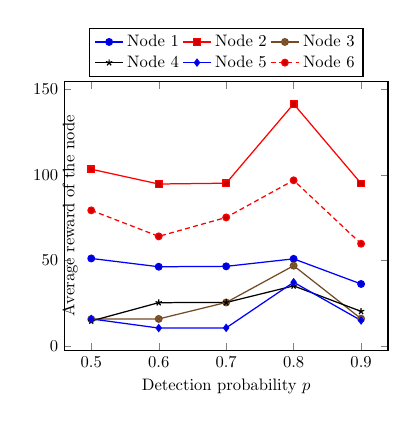
\begin{tikzpicture}[scale=0.6]
\begin{axis}[
  xlabel={Detection probability $p$},
  ylabel={Average reward of the node },
  y label style={at={(0.06,0.5)}},
  xtick={0.5,0.6,0.7,0.8,0.9,1.0},
  legend style={at={(0.5,1.2)},cells={align=right}, anchor=north,legend columns=3},
  grid style=dashed,
]

\addplot+[]
    coordinates {
(0.5,51.2408756424)(0.6,46.3989088055)(0.7,46.629281859)(0.8,51.0165854846)(0.9,36.3262102772)
};

\addplot+[]
    coordinates {
(0.5,103.390154828)(0.6,94.7445634867)(0.7,95.2136135648)(0.8,141.564157095)(0.9,95.0544799628)
};

\addplot+[]
    coordinates {
(0.5,15.7876437463)(0.6,15.9058652472)(0.7,25.5235856726)(0.8,47.0026051031)(0.9,16.0455657836)
};

\addplot+[]
    coordinates {
(0.5,14.6911918445)(0.6,25.4076999562)(0.7,25.5090975344)(0.8,35.2122191081)(0.9,20.3233753667)
};

\addplot+[]
    coordinates {
(0.5,15.9163072098)(0.6,10.573393829)(0.7,10.6704256682)(0.8,37.3424358141)(0.9,14.9838488261)
};

\addplot+[]
    coordinates {
(0.5,79.3520830459)(0.6,64.1507914239)(0.7,75.2190374666)(0.8,96.912552594)(0.9,59.8478399229)
};

\legend{Node 1, Node 2, Node 3, Node 4, Node 5, Node 6}
\end{axis}
\end{tikzpicture}

\caption{Scenario f)}
\label{fig:nodeimp_topo2_multiple}
\end{subfigure}
\caption{Results for single and multiple attackers - Scenarios e) and f)}
    \label{fig:mdp-result-topo2}
\end{figure}



\section{Determining the optimal monitoring nodes}
When solving a problem using an MDP, the solution is a dynamic proposition to choose actions as the system evolves.
However, from a technical aspect, the defender needs to have the nodes already monitoring the infrastructure before starting the migration process.
It becomes necessary to translate the dynamic answer of the MDP into a static \textit{a priori} deployment.
After determining the individual importance of each node, we propose to determine the optimal set of monitoring nodes.

The main difference is that each node was evaluated based on all the possible budget combinations, whereas what is defined here is a particular answer for a specific budget.
For each budget, the maximum reward is $\frac{b_f}{c_a} \sum\limits_{i \in \textbf{N}}V_i $ which corresponds to the corner case where the attacker never launched an attack, and we can evaluate the efficiency of the   monitoring nodes thanks to the associated reward.
Even if a particular monitoring set achieves close to the maximum reward, it is also because the set is tailored to a subset of all possible attacks.
We propose to determine the optimal monitoring state for each budget by weighting the reward they achieve with their occupation of the total solution space.

We note $S_{\text{abs}}$ the set of absorbing states, $S^{\text{Mo}}_{\text{abs}}$ the set of absorbing states with a common  monitoring set $Mo$, $\rho(Mo)$ the percentage of presence of set $Mo$ in the solution space and $R(Mo)$ the reward of monitoring set $Mo$.
% \begin{equation}
%     R(Mo) = \sum\limits_{s \in S_{Mo}^{abs}}\rho(Mo^s)R(Mo^s)
% \end{equation}
Then we propose to choose the optimal monitoring set $Mo^*$ with:
\begin{equation}
    Mo^* = \argmax\limits_{\text{Mo} \in S_{\text{abs}}} \left \{\sum\limits_{s \in S^{\text{Mo}}_{\text{abs}}}\rho(Mo^s)R(Mo^s) \right \}
\end{equation}

We present the results for in Table~\ref{tab:mdp-usecase-optiset}.


\textbf{Scenarios a) and b)\\}
We note that nodes 4 and 6 are always chosen in the monitoring.
Node 1 also often appears as a good candidate for a fourth node if it is not already chosen third.
With $p=0.7$ we observe that third and fourth nodes do not coincidate between (30,30) and (40,40) budgets.
This suggests that the combining two nodes increases their individual performance.
(Node 1 is surrounded by node 2 and 3 in the topology).
% This is explained because other budgets impact the individual importance of each node.

\textbf{Scenarios c) and d)\\}
One notable result is in scenario c) for $p=0.5,  (b_f,b_c) = (40,40)$ where the optimal monitoring set is 1,3 which could have two extra nodes ensuring the monitoring. However, it is worth noting that for $(b_f,b_c)=(30,30)$ the optimal set does not include node 2. The explanation comes from the fact that it takes less time to establish the path between the victim's network. The reward is based on the nodes of the attack path when the attack is completed. Therefore attacking extra nodes does not change the path and does not impact the reward. We conclude that the low detection probability coupled to a fullmesh topology may not be the ideal conditions to improve the security of the migration process.


\textbf{Scenarios e) and f)}\\
There is one  notable result, in scenario e) for $p=0.7,  (b_f,b_c) = (40,40)$ where the optimal monitoring set is 2,6 which could also have two extra nodes supporting the monitoring. In opposition to the counter-intuitive result of scenario c), we are here considering a higher detection percentage. Moreover, the nodes considered in this solution set are the nodes that see most of the attacks, one being the source of all attacks, and the other is part of the migrated virtual network and is communicating with almost all the other nodes in the infrastructure. The analysis of the optimal policy of this use case shows that part of the counter intuitive result is caused by removing either node 3 or 4 from the monitoring, which is understandable because it would not contribute to the detection of the remaining attacks. Removing monitoring here is equivalent to the action of doing nothing, with the unintended and unexpected upside of reducing the performance impact.
The other part of the counter intuitive result is due to removing node 6, the source of attacks from the monitoring. It is worth noting that this particular case represents a negligible portion of the solution space, and most of the counter intuitive result is due to the previous explanation. Considering that node 6 is removed at a point where the consequences of attacks will be minimal, we assume that removing the monitoring at this point was deemed equivalent to the do nothing action.


% Please add the following required packages to your document preamble:
% \usepackage{multirow}
% \usepackage{graphicx}
\begin{table}[]
\resizebox{\textwidth}{!}{%
\begin{tabular}{ccccccc}
\multicolumn{3}{c}{\textbf{Scenario a)}}                                                                     &                       & \multicolumn{3}{c}{\textbf{Scenario b)}}                                                                    \\ \cline{1-3} \cline{5-7} 
\multicolumn{1}{|c|}{p}                    & \multicolumn{1}{c|}{($b_f,b_c$)} & \multicolumn{1}{c|}{$Mo^*$}  & \multicolumn{1}{c|}{} & \multicolumn{1}{c|}{p}                    & \multicolumn{1}{c|}{($b_f,b_c$)} & \multicolumn{1}{c|}{$Mo^*$}  \\ \cline{1-3} \cline{5-7} 
\multicolumn{1}{|c|}{\multirow{2}{*}{0.5}} & \multicolumn{1}{c|}{(30,30)}     & \multicolumn{1}{c|}{2,4,6}   & \multicolumn{1}{c|}{} & \multicolumn{1}{c|}{\multirow{2}{*}{0.5}} & \multicolumn{1}{c|}{(30,30)}     & \multicolumn{1}{c|}{2,4,6}   \\ \cline{2-3} \cline{6-7} 
\multicolumn{1}{|c|}{}                     & \multicolumn{1}{c|}{(40,40)}     & \multicolumn{1}{c|}{1,2,4,6} & \multicolumn{1}{c|}{} & \multicolumn{1}{c|}{}                     & \multicolumn{1}{c|}{(40,40)}     & \multicolumn{1}{c|}{1,2,4,6} \\ \cline{1-3} \cline{5-7} 
\multicolumn{1}{|c|}{\multirow{2}{*}{0.7}} & \multicolumn{1}{c|}{(30,30)}     & \multicolumn{1}{c|}{1,4,6}   & \multicolumn{1}{c|}{} & \multicolumn{1}{c|}{\multirow{2}{*}{0.7}} & \multicolumn{1}{c|}{(30,30)}     & \multicolumn{1}{c|}{1,4,6}   \\ \cline{2-3} \cline{6-7} 
\multicolumn{1}{|c|}{}                     & \multicolumn{1}{c|}{(40,40)}     & \multicolumn{1}{c|}{2,3,4,6} & \multicolumn{1}{c|}{} & \multicolumn{1}{c|}{}                     & \multicolumn{1}{c|}{(40,40)}     & \multicolumn{1}{c|}{2,3,4,6} \\ \cline{1-3} \cline{5-7} 
\multicolumn{1}{|c|}{\multirow{2}{*}{0.9}} & \multicolumn{1}{c|}{(30,30)}     & \multicolumn{1}{c|}{4,5,6}   & \multicolumn{1}{c|}{} & \multicolumn{1}{c|}{\multirow{2}{*}{0.9}} & \multicolumn{1}{c|}{(30,30)}     & \multicolumn{1}{c|}{4,5,6}   \\ \cline{2-3} \cline{6-7} 
\multicolumn{1}{|c|}{}                     & \multicolumn{1}{c|}{(40,40)}     & \multicolumn{1}{c|}{1,4,5,6} & \multicolumn{1}{c|}{} & \multicolumn{1}{c|}{}                     & \multicolumn{1}{c|}{(40,40)}     & \multicolumn{1}{c|}{1,4,5,6} \\ \cline{1-3} \cline{5-7} 
                                           &                                  &                              &                       &                                           &                                  &                              \\
\multicolumn{3}{c}{\textbf{Scenario c)}}                                                                     &                       & \multicolumn{3}{c}{\textbf{Scenario d)}}                                                                    \\ \cline{1-3} \cline{5-7} 
\multicolumn{1}{|c|}{p}                    & \multicolumn{1}{c|}{($b_f,b_c$)} & \multicolumn{1}{c|}{$Mo^*$}  & \multicolumn{1}{c|}{} & \multicolumn{1}{c|}{p}                    & \multicolumn{1}{c|}{($b_f,b_c$)} & \multicolumn{1}{c|}{$Mo^*$}  \\ \cline{1-3} \cline{5-7} 
\multicolumn{1}{|c|}{\multirow{2}{*}{0.5}} & \multicolumn{1}{c|}{(30,30)}     & \multicolumn{1}{c|}{1,2,6}   & \multicolumn{1}{c|}{} & \multicolumn{1}{c|}{\multirow{2}{*}{0.5}} & \multicolumn{1}{c|}{(30,30)}     & \multicolumn{1}{c|}{1,3,6}   \\ \cline{2-3} \cline{6-7} 
\multicolumn{1}{|c|}{}                     & \multicolumn{1}{c|}{(40,40)}     & \multicolumn{1}{c|}{1,3}     & \multicolumn{1}{c|}{} & \multicolumn{1}{c|}{}                     & \multicolumn{1}{c|}{(40,40)}     & \multicolumn{1}{c|}{1,2,3,6} \\ \cline{1-3} \cline{5-7} 
\multicolumn{1}{|c|}{\multirow{2}{*}{0.7}} & \multicolumn{1}{c|}{(30,30)}     & \multicolumn{1}{c|}{1,3,6}   & \multicolumn{1}{c|}{} & \multicolumn{1}{c|}{\multirow{2}{*}{0.7}} & \multicolumn{1}{c|}{(30,30)}     & \multicolumn{1}{c|}{1,2,6}   \\ \cline{2-3} \cline{6-7} 
\multicolumn{1}{|c|}{}                     & \multicolumn{1}{c|}{(40,40)}     & \multicolumn{1}{c|}{1,2,3,6} & \multicolumn{1}{c|}{} & \multicolumn{1}{c|}{}                     & \multicolumn{1}{c|}{(40,40)}     & \multicolumn{1}{c|}{1,2,5,6} \\ \cline{1-3} \cline{5-7} 
\multicolumn{1}{|c|}{\multirow{2}{*}{0.9}} & \multicolumn{1}{c|}{(30,30)}     & \multicolumn{1}{c|}{1,3,6}   & \multicolumn{1}{c|}{} & \multicolumn{1}{c|}{\multirow{2}{*}{0.9}} & \multicolumn{1}{c|}{(30,30)}     & \multicolumn{1}{c|}{1,2,6}   \\ \cline{2-3} \cline{6-7} 
\multicolumn{1}{|c|}{}                     & \multicolumn{1}{c|}{(40,40)}     & \multicolumn{1}{c|}{1,2,3,6} & \multicolumn{1}{c|}{} & \multicolumn{1}{c|}{}                     & \multicolumn{1}{c|}{(40,40)}     & \multicolumn{1}{c|}{1,2,3,6} \\ \cline{1-3} \cline{5-7} 
                                           &                                  &                              &                       &                                           &                                  &                              \\
\multicolumn{3}{c}{\textbf{Scenario e)}}                                                                     &                       & \multicolumn{3}{c}{\textbf{Scenario f)}}                                                                    \\ \cline{1-3} \cline{5-7} 
\multicolumn{1}{|c|}{p}                    & \multicolumn{1}{c|}{($b_f,b_c$)} & \multicolumn{1}{c|}{$Mo^*$}  & \multicolumn{1}{c|}{} & \multicolumn{1}{c|}{p}                    & \multicolumn{1}{c|}{($b_f,b_c$)} & \multicolumn{1}{c|}{$Mo^*$}  \\ \cline{1-3} \cline{5-7} 
\multicolumn{1}{|c|}{\multirow{2}{*}{0.5}} & \multicolumn{1}{c|}{(30,30)}     & \multicolumn{1}{c|}{2,3,6}   & \multicolumn{1}{c|}{} & \multicolumn{1}{c|}{\multirow{2}{*}{0.5}} & \multicolumn{1}{c|}{(30,30)}     & \multicolumn{1}{c|}{1,2,6}   \\ \cline{2-3} \cline{6-7} 
\multicolumn{1}{|c|}{}                     & \multicolumn{1}{c|}{(40,40)}     & \multicolumn{1}{c|}{1,2,3,6} & \multicolumn{1}{c|}{} & \multicolumn{1}{c|}{}                     & \multicolumn{1}{c|}{(40,40)}     & \multicolumn{1}{c|}{1,2,3,6} \\ \cline{1-3} \cline{5-7} 
\multicolumn{1}{|c|}{\multirow{2}{*}{0.7}} & \multicolumn{1}{c|}{(30,30)}     & \multicolumn{1}{c|}{2,3,6}   & \multicolumn{1}{c|}{} & \multicolumn{1}{c|}{\multirow{2}{*}{0.7}} & \multicolumn{1}{c|}{(30,30)}     & \multicolumn{1}{c|}{1,2,6}   \\ \cline{2-3} \cline{6-7} 
\multicolumn{1}{|c|}{}                     & \multicolumn{1}{c|}{(40,40)}     & \multicolumn{1}{c|}{2,6}     & \multicolumn{1}{c|}{} & \multicolumn{1}{c|}{}                     & \multicolumn{1}{c|}{(40,40)}     & \multicolumn{1}{c|}{1,2,3,6} \\ \cline{1-3} \cline{5-7} 
\multicolumn{1}{|c|}{\multirow{2}{*}{0.9}} & \multicolumn{1}{c|}{(30,30)}     & \multicolumn{1}{c|}{2,3,6}   & \multicolumn{1}{c|}{} & \multicolumn{1}{c|}{\multirow{2}{*}{0.9}} & \multicolumn{1}{c|}{(30,30)}     & \multicolumn{1}{c|}{1,2,6}   \\ \cline{2-3} \cline{6-7} 
\multicolumn{1}{|c|}{}                     & \multicolumn{1}{c|}{(40,40)}     & \multicolumn{1}{c|}{2,3,5,6} & \multicolumn{1}{c|}{} & \multicolumn{1}{c|}{}                     & \multicolumn{1}{c|}{(40,40)}     & \multicolumn{1}{c|}{1,2,4,6} \\ \cline{1-3} \cline{5-7} 
\end{tabular}%
}
\caption{Optimal monitoring sets of the Use Cases}
\label{tab:mdp-usecase-optiset}
\end{table}

\section{Discussion}
% \GB{you do not discuss the complexity limitation of your MDP. I think it is important and honest to point it out.}
\label{sec:mdp-discussion}
The evaluation of our model has outlined several technical and modeling limitations:

First of all, the use of budgets as part of the MDP state is a root cause for the complexity in generating the MDP states. Indeed, these budgets act as a sort of ``identifiers`` that make the number of states grow exponentially depending on the budgets.
Secondly, the use of the duration of the migration in the description of each state of the MDP limits the capacities of the attacker. Indeed, the model implies that once the migration if finished the attacker cannot attack the infrastructure anymore. This raises the question ``What is a realistic time frame for the attacker to compromise the migration process and the virtual network ?".
In some numerical applications we have extended the duration of the migration to one extra iteration ($b_c = 40$ ). This has given the opportunity for the attack to extend his attack and reach more nodes.
Because the infrastructure is vulnerable to the attack model described in Section~\ref{sec:attack_model}, it is reasonable to assume that the attacker will keep attacking the infrastructure after the end of the migration. For instance, he may continue to establish his path if he could not complete it prior the end of the migration.
We can generalize the previous point to a global question: ``When representing the behaviour of an external element in the MDP, which aspect of the MDP should include the modeling?". While the formalism does not set any hard limitation, it is important to consider the realism aspect of the modeling with regard to practical scenarios and the threat model used. We represented our attacker in the definition of the states as well as the reward function, since rewards are based on the progression of the attack.
The use cases we proposed did not distinguish virtual networks between one-to-one mapping and one-to-many mapping. While arbitrary topologies are an important feature of a virtualization service, in our model we can easily alleviate this issue because physical nodes embedding virtual resources are part of the migration.




\section{General Conclusion}
\label{sec:mdp-conclusion}
In this chapter, we investigated the Resource Allocation problem in a security context. Our objective was to determine which nodes of the infrastructure should be performing monitoring tasks to detect attacks against the migration process.
We proposed a Markovian Decision Process to represent how an infrastructure provider can solve this RA problem and find out the optimal choices.
We introduced the attacker in the definition of the model, which is rarely done from a security perspective. Indeed, MDPs are often modeling only one agent to interact with the system, but the inclusion of an actor of a different nature is generally not considered.
We also provided an experimental prototype for the MDP generation, solving and results analysis  (\url{https://github.com/FabienCharmet/MDPRA}).
Results show that we can determine which nodes provide the best security with regard to current attacks, as well as how the dynamic aspect of the optimal policy can be translated into an \textit{a priori} deployment of the monitoring resources on the nodes.
When the attacker can launch attacks from several sources, the impact of the nodes on the monitoring is much more differentiated and gives a better understanding of their role in the infrastructure.
We also ran the simulations on several network topologies to evaluate the impact of the attack routing on the optimal solution. Results show that a full-mesh topology is more complex to defend because of the multitude of attack paths.
% Markov Decision Processes are rarely used for a resource allocation problem in a security context.

We advocate that the flexibility of the MDP formalism can be leveraged to dynamically recompute the destination substrate while the migration is ongoing.
Instead of deciding where to deploy the monitoring, the migration process would use the MDP to predict the target of the next attack and should recompute the embedding of the VN if the next virtual node will be embedded on a compromised physical node. The approach would give additional flexibility to the VNE algorithm and make it more secure. We emphasize on the Reinforcement Learning aspect of this approach, which could be extended by using a Q-Learning model where the defender does not know precisely which nodes have been attacked.
\GB{this becomes a Reinforcement Learning approach, right?}\FC{MDP is RL in the first place} \CK{Il n'y a pas vraiment d'idee d'apprentissage dans ce que l'on fait. C'est interessant de souligner l'aspect apprentissage renforce de l'evolution que tu proposes}\FC{Je rajoute l'aspect apprentissage de l'evolution, mais je souligne que le MDP est un formalisme de reinforcement learning. L'aspect RL dans notre cas est moins visible car on a pas de Q-Learning. Mais il me semble qu'au sens strict du terme on fait du RL parce que l'on utilise un MDP}

